\documentclass{report}

\usepackage{graphicx}
\usepackage{epstopdf}
\usepackage{amsmath}
\usepackage{amssymb}
\usepackage{amsthm}
\usepackage{algorithm, algpseudocode}
\usepackage{caption}
\usepackage{url}

\newcommand{\rr}[0]{\mathbf{r}}
\newcommand{\xx}[0]{\mathbf{x}}
\newcommand{\ud}{\,\mathrm{d}}
\newcommand{\comment}[1]{}

\begin{document}
\title{Asymptotic Statistics of Nodal Domains of Quantum Chaotic Billiards in the Semiclassical Limit}
\author{Kyle Konrad\\
  Dartmouth College\\
  Computer Science Department\\
  Advisor: Alex Barnett}
\date{\today}

\maketitle

\begin{abstract}
  Quantum chaos concerns eigenfunctions of the Laplace operator in a domain where a billiard ball would bounce chaotically.
Such chaotic eigenfunctions have been conjectured to share statistical properties of their nodal domains with a simple percolation model, from which many interesting quantities can be computed analytically. We numerically test conjectures on the number and size of nodal domains of quantum chaotic eigenfunctions at very high energies, approaching the semiclassical limit. We use a highly efficient scaling method to quickly compute eigenfunctions at low resolution and interpolate to higher resolution. We computed $10^{5}$ eigenfunctions and counted $10^{9}$ nodal domains. Our results agree with the conjectured size nodal domains but disagree with the conjectured mean and variance of the number of nodal domains.
\end{abstract}

\chapter{Introduction}
\label{chap:intro}
\section{Motivation}
\label{sec:motivation}
Nodal domains characterize regions of a vibrational surface (e.g. a drum head) that move in phase. The boundaries between nodal domains, known as nodal lines, are the regions which do not vibrate at all (fig. \ref{fig:drum}). Understanding the characteristics of nodal domains has applications in spectral geometry, mathematical physics, mechanical engineering, geophysics, astrophysics, and many other area dealing with wave behavior \cite{wigman}.

\begin{figure}
  \begin{center}
    \includegraphics[width=\textwidth]{figs/drum/2_3_mode_side_view.eps}
    \caption{A circular vibrational surface with nodal lines shown in black. Nodal domains are regions between black lines}
    \label{fig:drum}
  \end{center}
\end{figure}

We study nodal domains of eigenfunctions of the Laplace operator on nonintegrable Euclidean domains, or chaotic billiards. These eigenfunctions are known as quantum chaotic eigenfunctions because they are solutions of the quantum mechanical wave equation, the Schr\"{o}dinger equation. Quantum chaotic eigenfunctions are a canonical example of quantum chaos, which lies at the intersection of quantum mechanics and chaos theory. The primary signature of chaos in classical systems is a nonlinear (exponential) divergence of trajectories in the phase space of a system. Quantum mechanics however, is entirely linear and quantum chaos deals with energy eigenfunctions of systems, which are constant in time. Thus chaos in quantum systems is manifest in different ways, one of the most studied being wavefunctions in chaotic domains. Figure \ref{fig:classical_vs_quantum} shows a classical orbit and a quantum eigenfunction on the same billiard.

\begin{figure}
  \begin{center}
    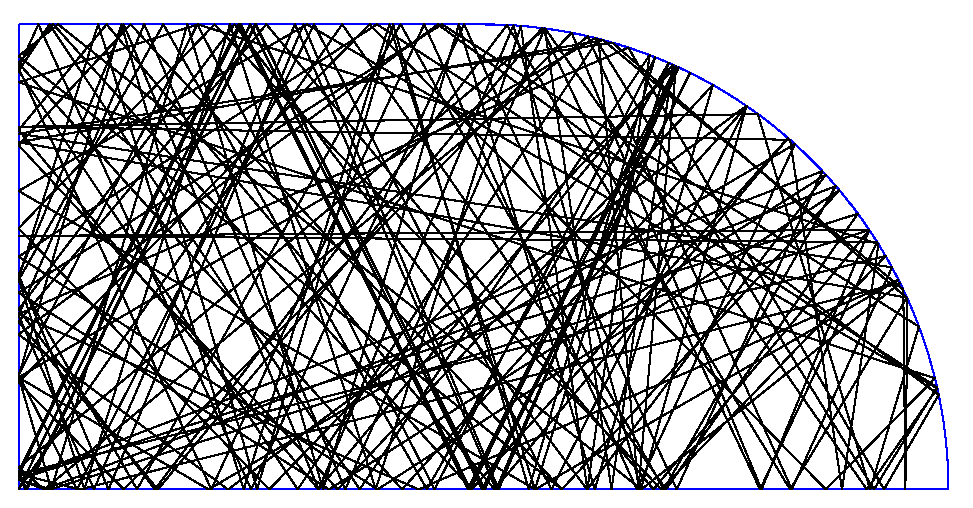
\includegraphics[width=\textwidth]{figs/classical/stadium_orbit.eps}
    \linebreak
    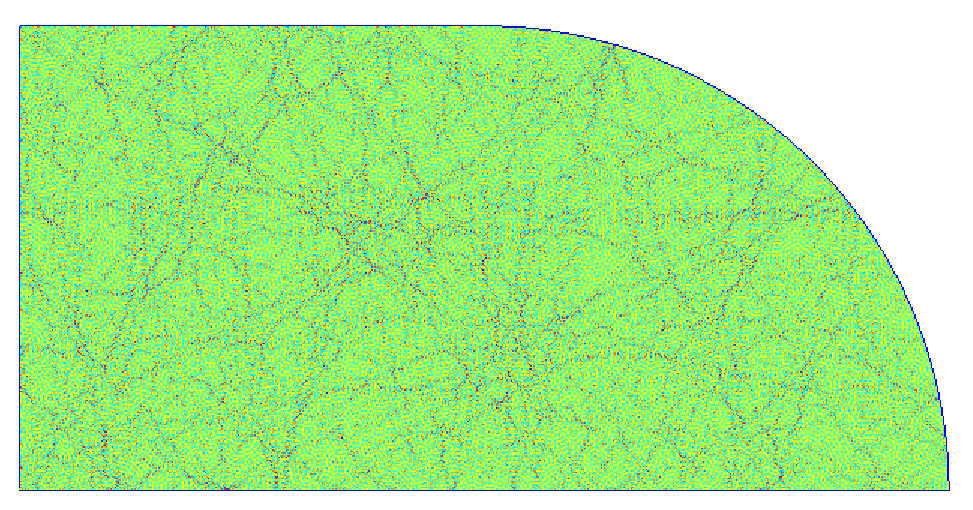
\includegraphics[width=\textwidth]{figs/classical/stadium_eigenfunction.eps}
    \linebreak
    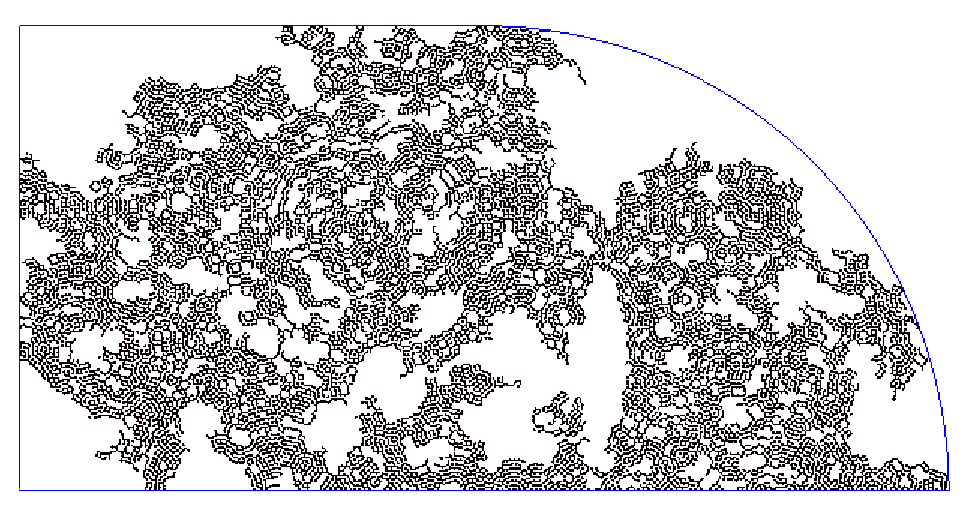
\includegraphics[width=\textwidth]{figs/classical/stadium_eigenfunction_largest_nodal_domain.eps}
    \caption{Above: A classical orbit in a billiard; center: a quantum eigenfunction in the same billiard; below: the largest nodal domain in the center eigenfunction.}
    \label{fig:classical_vs_quantum}
  \end{center}
\end{figure}

The goal of this project is to numerically test conjectures on the mean and variance of the number and sizes of nodal domains in quantum chaotic eigenfunctions in the high energy, or semiclassical, limit. These tests are motivated by questions from number theorist Peter Sarnak, who inspired us to test the conjecture on the mean number of nodal domains. Obtaining relevant data requires solving new computational challenges due to the computational intensity of evaluating eigenfunctions at very high energies. We hope these results will enable further mathematical investigation of eigenfunctions and that the tools developed herein may be applied to related problems in quantum chaos.

\section{Classical Chaos in Billiards}
\label{sec:classical}
A billiard is a compact domain $\Omega \subset \mathbb{R}^{2}$. By parameterizing the perimeter of a billiard by $s \in [0,L)$, where $L$ is the perimeter length, we can construct a map $P: \mathbb{R} \pmod{L} \times \mathbb{R} \pmod{\pi} \rightarrow \mathbb{R} \pmod{L} \times \mathbb{R} \pmod{\pi}$ such that a trajectory incident on the boundary at parameter $s$ and angle $\theta$ from the tangent to the boundary at $s$ will next intersect the boundary at parameter and angle of incidence $(s', \theta') = P(s, \theta)$. This map describes the motion of a ball bouncing in the domain $\Omega$.

Chaos in classical systems is characterized by the Lyapunov exponent $\lambda$ of a system, which describes how quickly nearby trajectories diverge. It is computed as the long time ratio of the divergence of two initially close paths:
\[
\lambda = \lim_{n \to \infty} \lim_{\vert \boldsymbol\epsilon \vert \to 0} \frac{1}{n} \ln{\frac{\vert P^{n}({\bf x_{0}}) - P^{n}({\bf x_{0}} + \boldsymbol\epsilon) \vert}{\vert \boldsymbol\epsilon \vert}}
\]
Where ${\bf x_{0}} = (s_{0}, \theta_{0})$ and $\vert (s, \theta) \vert = s$. From this definition it follows that
\[
\vert P^{n}({\bf x_{0}}) - P^{n}({\bf x_{0}} + \boldsymbol\epsilon) \vert \approx e^{\lambda n} \vert \boldsymbol\epsilon \vert
\]
for small $\boldsymbol\epsilon$ and large $n$. Thus a tiny change $\boldsymbol\epsilon$ in initial conditions produces a change that grows exponentially over time with growth rate $\lambda$. Chaotic systems have a positive Lyapunov exponent and therefore have unpredictable long-term behavior because arbitrarily small errors in measurements of initial conditions eventually become large. As these errors grow to the size of the domain, the position of a particle approaches a uniform distribution over the entire billiard. The property that small subsets of $\Omega$ eventually map to all of $\Omega$ is known as ergodicity (see appendix \ref{sec:ergodicity} for a formal definition).

\section{Quantum Chaos in Billiards}
\label{sec:billiards}
A quantum wave-particle in a billiard $\Omega$ obeys the Schr\"odinger equation
\[
E u(\rr) = - \frac{\hbar^{2}}{2m} \Delta u(\rr) + V(\rr) u(\rr)
\]
Where $\Delta = \nabla^{2} = \frac{\partial^{2}}{\partial x^{2}} + \frac{\partial^{2}}{\partial y^{2}}$ is the Laplacian differential operator in two dimensions. Setting $\hbar = 2m = 1$ and $V(\rr) = 0$ for $\rr \in \Omega$ while enforcing Dirichlet boundary conditions $u(\rr) = 0$ for $\rr \in \Gamma = \partial \Omega$ simplifies this to the Helmholtz equation
\begin{equation}
\label{eq:helmholtz}
\begin{cases}
(\Delta + k^{2})u(\rr) = 0 & \text{if } \rr \in \Omega\\
  u(\rr) = 0 & \text{if } \rr \in \Gamma
\end{cases}
\end{equation}
where $k^{2} = E$ is the corresponding eigenvalue for eigenfunction $u(\rr)$ and $E$ is kinetic energy of the quantum wave-particle.

We focus our investigation on two billard shapes: the generalized rectangular Sinai billiard and the Stadium billiard (fig. \ref{fig:billiards}). In both cases we desymmetrize the billard shapes by considering only a quarter of the full shape. This restricts our basis set to functions that are odd as functions of x and y, i.e., $f(-x,y) = f(x,-y) = -f(x,y)$.

\begin{figure}
  \begin{center}
    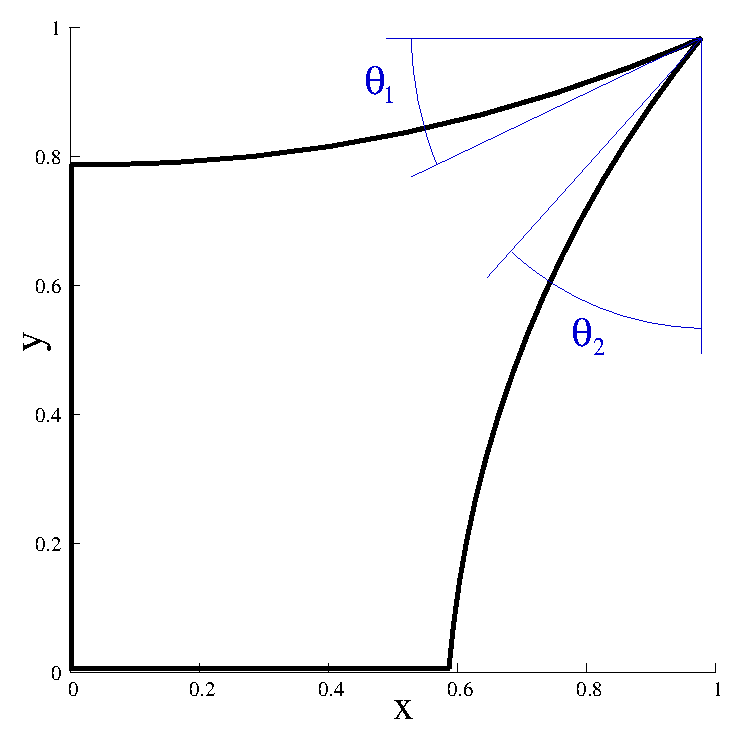
\includegraphics[width=0.3\textwidth]{figs/domains/qugrs_fig.eps}
    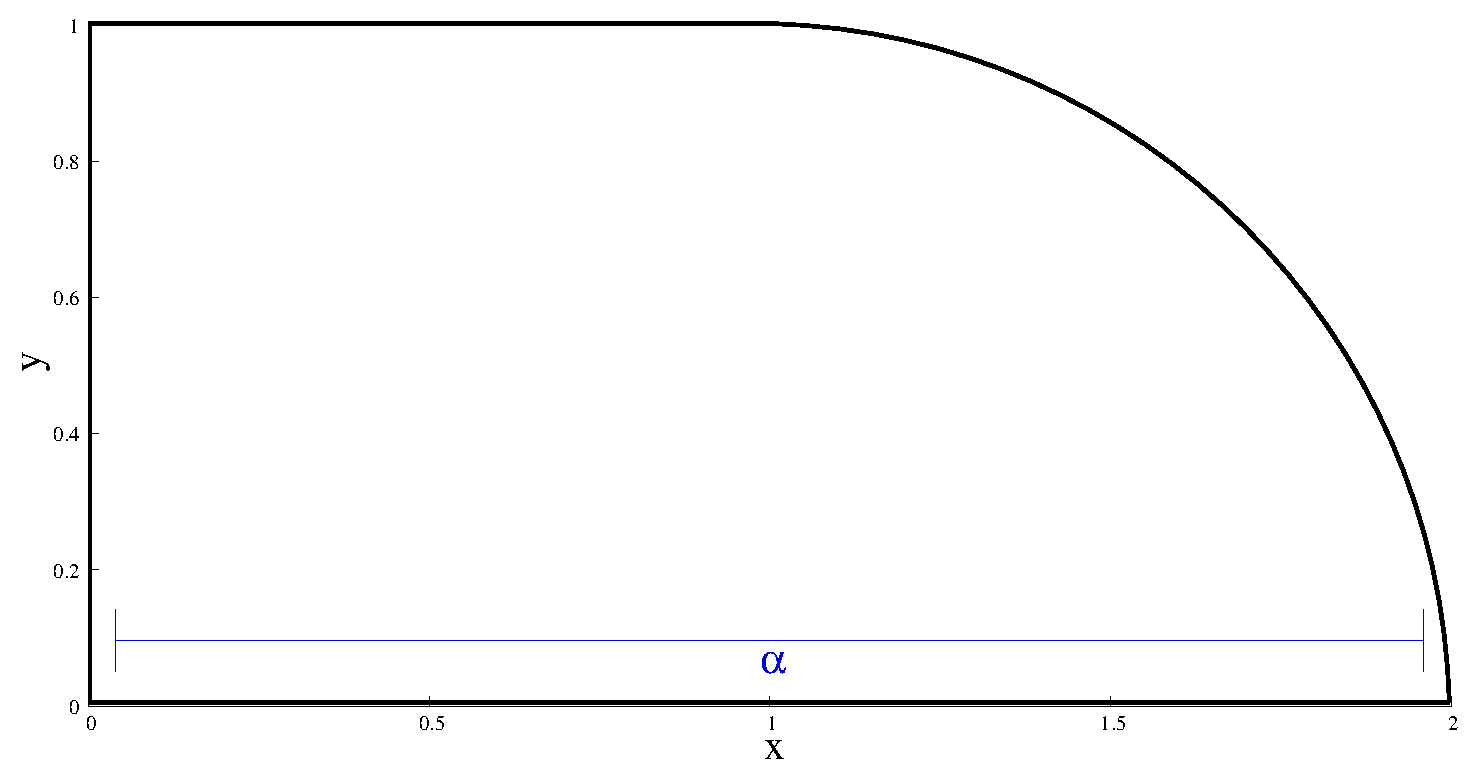
\includegraphics[width=0.6\textwidth]{figs/domains/qust_fig.eps}
    \caption{Left: quarter generalized rectangular Sinai billiard; right: quarter stadium billiard}
    \label{fig:billiards}
  \end{center}
\end{figure}

The Sinai billiard is constructed from circular arcs that meet at $(1,1)$ and is parameterized by two angles, $\theta_{1}$ and $\theta_{2}$, the angles from horizontal and vertical, respectively, of the arcs at $(1,1)$. The Sinai billiard is said to demonstrate ``hard chaos'' because there are no stable or neutrally stable orbits. We use values of $\theta_{1} = 0.4$ and $\theta_{2} = 0.7$.

The stadium billiard is constructed from a rectangular region and a quarter circle and is parameterized by the the horizontal length of the billiard $\alpha$. We use a value of $\alpha = 2$ here. The stadium billiard contains neutrally stable orbits, specifically those with vertical momentum in the rectangular region. Neutrally stable orbits have zero Lyapunov exponent but any perturbation will cause them to have positive Lyapunov exponenet. The existence of such orbits implies that the stadium does not demonstrate hard chaos but because these orbits occupy a measure zero subset of phase space, the stadium still has chaotic properties. These classical orbits are manifest in quantum eigenfunctions as so-called ``bouncing-ball'' modes (fig. \ref{fig:bouncing_ball_mode}).

\begin{figure}
  \begin{center}
    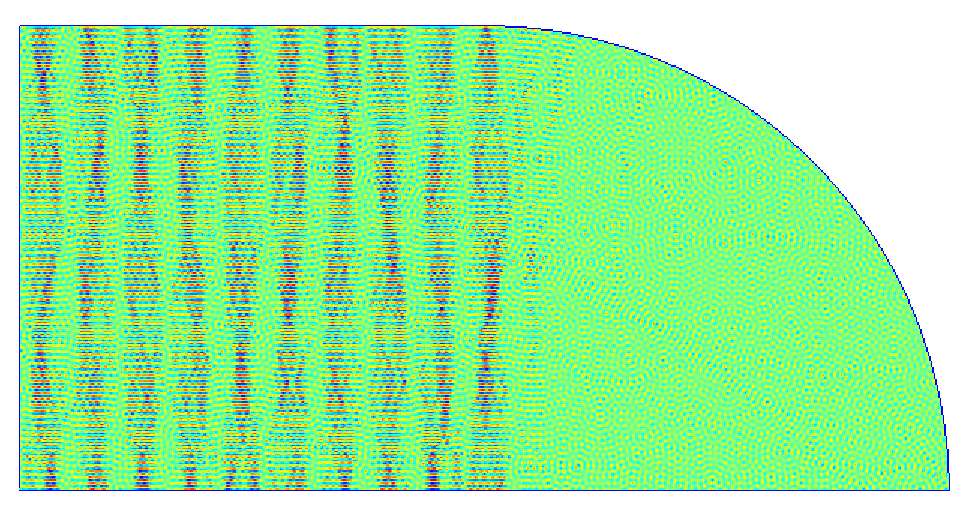
\includegraphics[width=\textwidth]{figs/classical/stadium_eigenfunction_bouncing_ball_mode.eps}
    \caption{A bouncing ball mode in the stadium billiard with $k = 500.3881$}
    \label{fig:bouncing_ball_mode}
  \end{center}
\end{figure}

\section{Percolation Model}
\label{sec:percolation}
Bogomolny and Schmit \cite{bogomolny} have argued that nodal domains of random functions (which are considered an accurate proxy for eigenfunctions of chaotic systems \cite{heller}) can be modeled by nodal domains of a percolation model. Their percolation model is formed by creating a checkerboard of positive and negative regions with a grid size given by the average spacing of zeros of random functions along a particular axis. This checkerboard pattern can be realized as an eigenfunction $\bar{u}(x,y) = sin(\frac{kx}{\sqrt{2}})sin(\frac{ky}{\sqrt{2}})$ of a square billiard $\Omega = [0,1]^{2}$. A random eigenfunction can be modelled as this mean eigenfunction $\bar{u}(x,y)$ plus another term representing deviation from the mean $u(x,y) = \bar u(x,y) + \delta u(x,y)$. The deviation term $\delta u(x,y)$ is modelled by perturbing each nodal line crossing by connecting two diagonal regions (fig. \ref{fig:percolation}). The decision of which nodal domains to connect is made randomly with equal probability for either possibility.

\begin{figure}
  \begin{center}
    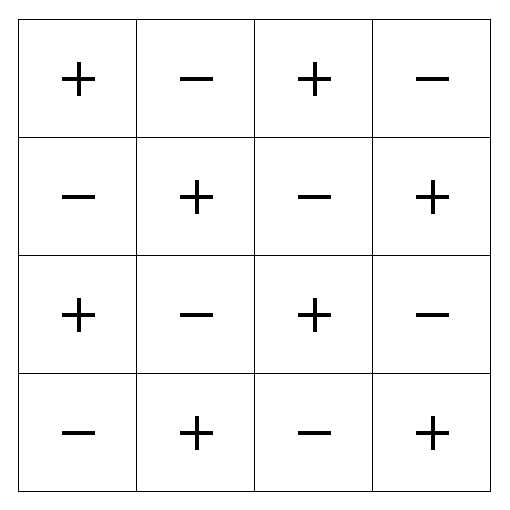
\includegraphics[width=0.4\textwidth]{figs/percolation/checkerboard.eps}
    \hspace{1 cm}
    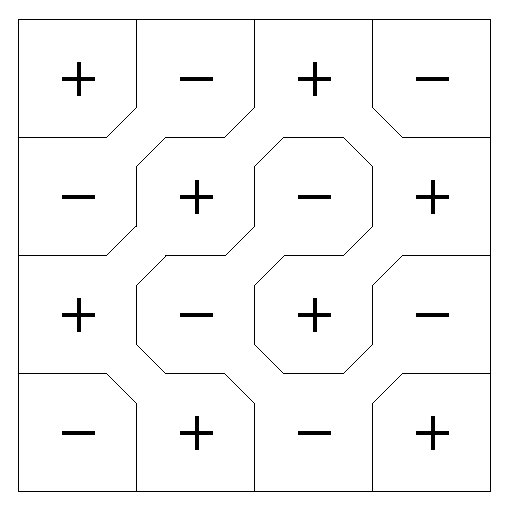
\includegraphics[width=0.4\textwidth]{figs/percolation/perturbed.eps}
    \caption{Left: checkerboard pattern; right: perturbed checkerboard pattern}
    \label{fig:percolation}
  \end{center}
\end{figure}

Bogomolny and Schmit apply results from graph theory and statistical physics to compute the distribution of nodal domains in this percolation model. These results comprise the conjectures we seek to test numerically.

\newtheorem{conj}{Conjecture}
\begin{conj}[Mean of Nodal Domain Count]
  \label{conj:mean}
  The number of nodal domains $\nu(E)$ in a quantum chaotic eigenfunction with energy $E$ is normally distributed with mean
  \begin{equation}
    \frac{\bar{\nu}(E)}{\bar{N}(E)} = \frac{3 \sqrt{3} - 5}{\pi} \approx 0.0624
  \end{equation}
\end{conj}

\begin{conj}[Variance of Nodal Domain Count]
  \label{conj:variance}
  The number of nodal domains $\nu(E)$ in a quantum chaotic eigenfunction with energy $E$ is normally distributed with variance
  \begin{equation}
    \frac{\sigma^{2}(\nu(E))}{\bar{N}(E)} = \frac{18}{\pi^{2}} + \frac{4 \sqrt{3}}{\pi} - \frac{25}{2 \pi} \approx 0.0502
  \end{equation}
\end{conj}  

In both conjectures, $\bar{N}(E)$ is the mean number of eigenvalues less than $E$ which has asymptotic behavior given by Weyl's law \cite{garabedian}
\begin{equation}
  \label{eq:weyl}
  \bar{N}(E) \sim \frac{\vert \Omega \vert E}{4 \pi}
\end{equation}

Bogolmony and Schmit also obtain a prediction for the distribution of areas of nodal domains.

\begin{conj}[Area of Nodal Domains]
  \label{conj:area}
  The area $s$ of nodal domains in a quantum chaotic eigenfunction follows the distribution
  \begin{equation}
    f(s) \propto s^{-\tau}
  \end{equation}
  where $\tau = \frac{187}{91}$ is the Fisher exponent.
\end{conj}

\subsection{Implementation}
The percolation model was implemented in code by creating a checkerboard pattern with each square being two pixels by two pixel that was then perturbed at each nodal line crossing by changing the sign of a pixel to either connect the top right square to the bottom left square or the top left square to the bottom right square (fig. \ref{fig:percolation_implementation}). The number of squares $m$ in one direction on a unit grid is determined by $k$ to be \cite{bogomolny}.
\[
m = \frac{k}{\sqrt{2}\pi}
\]

\begin{figure}
  \begin{center}
    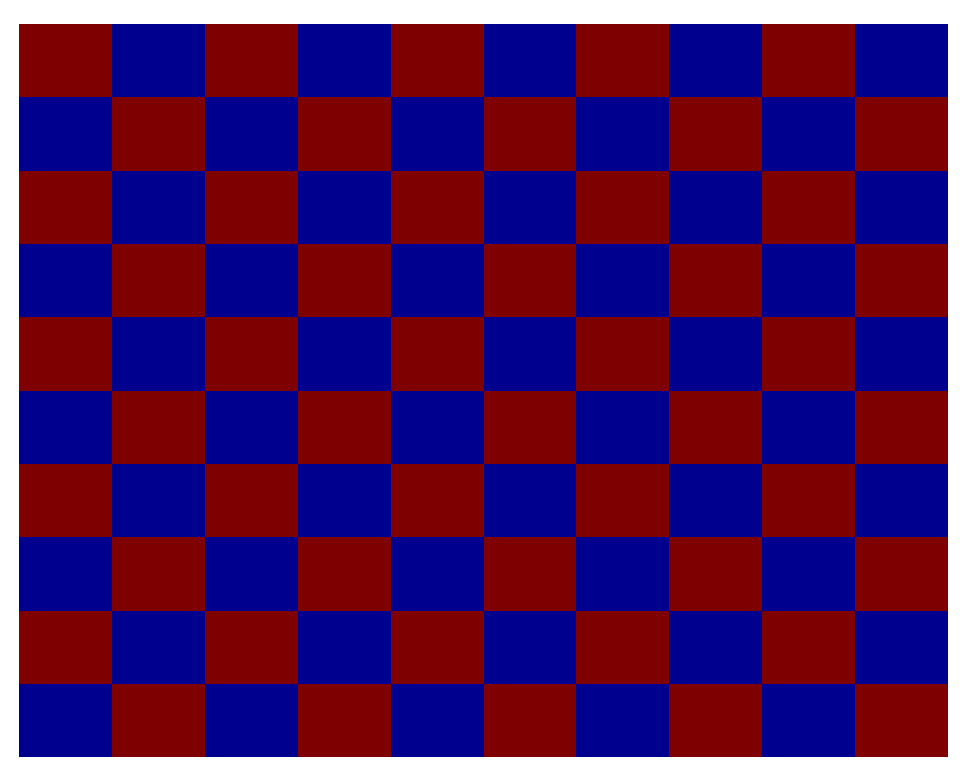
\includegraphics[width=0.4\textwidth]{figs/percolation/checkerboard_implementation.eps}
    \hspace{1 cm}
    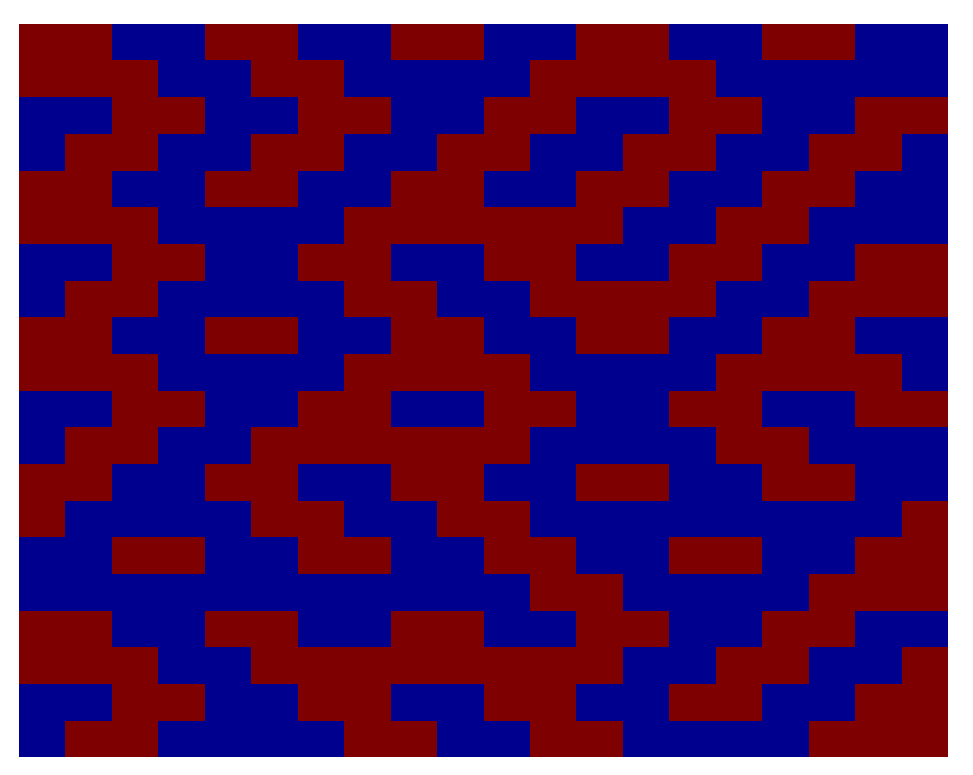
\includegraphics[width=0.4\textwidth]{figs/percolation/perturbed_implementation.eps}
    \caption{Left: checkerboard pattern implementation; right: perturbed checkerboard pattern implementation}
    \label{fig:percolation_implementation}
  \end{center}
\end{figure}

Making each square two pixels by two pixels uses a grid of size $(2m)^{2} = \frac{2 k^{2}}{\pi^2}$. This construction allows us to numerically validate the conjectures of the percolation model via the nodal domain counting algorithm described in \ref{sec:counting}.

\section{Random Plane Waves}
A random superposition of plane waves,
\begin{equation}
  \label{eq:rpw}
  u_{rand}(\rr ; k) = \Re \left[ \lim_{N \rightarrow \infty} \frac{1}{\sqrt{N}} \sum_{n=1}^{N} \omega_{n} \exp{\left\{\mathrm{i} k \hat{n}_{n} \cdot \rr \right\}} \right]
\end{equation}
where $\omega_{n} \sim \mathcal{N}(0,1)$ are complex and independent and identicially distributed and $\hat{n}_{n} = (\cos \frac {2 \pi n}{N}, \sin \frac {2 \pi n}{N})$ are evenly spaced vectors around the unit circle, is considered an accurate model for a quantum chaotic eigenfunctions \cite{heller}. This random superposition of plane waves (hereafter ``random plane wave'') is built from plane waves with constant wavenumber $k$ with random phase and amplitude, oriented in all directions.

Numerically, random plane waves can be computed quickly using a nonuniform fast Fourier transform on vectors of length $k$ with random phase. When testing new methods or obtaining general statistics, we often use random plane waves in place of actual eigenfunctions to save computation time.

\chapter{Methods}
\section{Computation of Eigenfunctions via Scaling Method}
\label{sec:scaling_method}
\subsection{Theory}
Vergini and Saraceno \cite{vergini} developed a method of computing high energy eigenfunctions of chaotic billiards using a scaling method. The method simultaneously finds all eigenfunctions $u_{i}(\rr)$ with wavenumber in a given window $[k - \Delta k, k + \Delta k]$ by scaling each eigenfunction. The scaled eigenfunctions $\chi_{i}(k, \rr)$ are computed as
\[
\chi_{i}(k, \rr) = u_{i} \left( \frac{k}{k_{i}} \rr \right)
\]
This scaling causes all eigenfunctions to fall approximately in a linear subspace of a single basis set $\left\{ \xi_{l} \right\}_{l=1}^{B}$,
\[
\chi_{i}(k, \rr) = \sum_{l=1}^{B} h_{l}^{(i)} \xi_{l}(k, \rr) + \epsilon_{i}(\rr)
\]
where $\epsilon_{i}(\rr) \ll 1$ for sufficiently large $B$, the number of basis functions used. Values of $B$ of approximately $1.5 \frac{k \vert \Gamma \vert}{\pi}$ have been shown to produce $\epsilon < 10^{-4}$ \cite{barnett_hassell}. This single basis set provides a significant efficiency gain over prior methods because many eigenfunctions can be found by solving a single linear system and evaluating a single basis set on the domain.

The choice of basis functions $\xi_{l}(k, \rr)$ depend on the billiard shape being used. For the quarter generalized rectangular Sinai billiard the basis set consists of fundamental solutions, or irregular Bessel functions, (which satisfy $(\Delta + k^2)\xi_{l}(k, \rr) = 0$) placed along $\Gamma^{+}$, the set of points ouside $\Omega$ whose nearest distance to $\Gamma$ is $D$ where $kD$ is taken to be $7$ so that $D$ is approximately one wavelength. For the quarter stadium, the basis set is plane waves with orientations evently spaced around the circle.

The numerical implementation of the scaling method is based on solving a generalized eigenvalue problem from which one can reconstruct eigenvalues and eigenfunctions of the original Dirchlet boundary value problem. The basic approach is to construct $B$ by $B$ matrices ${\bf F}$ and ${\bf G}$ where
\[
{\bf F}_{ij} = \langle \xi_{i}, \xi_{j} \rangle
\] 
and
\[
{\bf G}_{ij} = \left( \langle \xi_{i}, x \cdot \nabla \xi_{j} \rangle + \langle x \cdot \nabla \xi_{i}, \xi_{j} \rangle \right) / k
\]
By solving the generalized eigenvalue problem
\[
{\bf F} h = \mu {\bf G} h
\]
one obtains approximations of the eigenvalues of the original problem with
\[
\hat{k}_{i} = k - 2/\mu_{i}
\]
and approximate eigenfunctions by ``undilating'' the generalized eigenvectors
\begin{equation}
  \label{eq:uhat}
  \hat{u}_{i}(\rr) = \sum_{l=1}^{B} h_{l} \xi_{l}(\hat{k}, \rr)
\end{equation}

The scaling method runs in $O(B^{3}) = O(k^{3})$ time \cite{barnett} and approximates eigenvalues and eigenfunctions with error $O({\Delta k}^{3})$ \cite[p. 32]{barnett_hassell}.

\subsection{Eigenfunction evaluation}
The scaling method only computes coefficients of basis functions, which must be evaluated in order to obtain eigenfunction values at arbitrary $\rr \in \Omega$. One method is to evaluate $\hat{u}(\rr)$ as in (\ref{eq:uhat}), but this requires evaluating the basis functions $\xi_{l}(\hat{k}, \rr)$ for each approximate eigenvalue $\hat{k}$. For efficiency, we instead evaluate only $\xi_{l}(k, \rr)$, which produces a dilated eigenfunction that can be transformed back to $\hat{u}$ by dilating the coordinate system. Thus we can evaluate all eigenfunctions in the energy window with $NB$ basis function evaulations and $nNB$ coefficient multiplications, where $n$ is the number of eigenfunctions in the energy window, $N$ is the number of evaluation points, and $B$ is the number of basis functions. Basis evaluation are much more expensive than multiplications; table \ref{tab:eval_ratios} summarizes the ratios of these costs.

\begin{table}
  \centering
  \begin{tabular}{|r|c|c|}
    \hline
    Billiard & Ratio & $k_c$ \\ \hline
    \hline
    Sinai & 75 & 3860 \\ \hline
    Stadium & 31 & 550 \\
    \hline
  \end{tabular}
  \caption{Ratios of basis function evaluation time to coefficient multiplication time for various billiards. Column $k_c$ contains the value of $k$ for which $n$ is equal to the given ratio with $\Delta k = 0.1$ and coefficient multiplications take as long as evaluating basis functions}
  \label{tab:eval_ratios}
\end{table}

As noted above, errors in eigenfunctions produced by the scaling method scale like $O({\Delta k}^{3})$ and are independent of $E$ so we use a constant $\Delta k$. We estimate errors by calculating the tension
\[
t = \left( \int_{\Gamma} u(\rr)^{2} d\rr \right)^{\frac{1}{2}}
\]
$\Delta E$ is chosen such that $t \lesssim 10^{-4}$. Using Weyl's law \ref{eq:weyl} we can obtain an estimate of the number of eigenfunctions in an energy window to be
\[
n \approx \frac{\vert \Omega \vert}{4 \pi} ((E + \Delta E) - (E - \Delta E)) = \frac{\vert \Omega \vert}{2 \pi} \Delta E
\]

We choose $\Delta k$ to be as large as possible while keeping errors small in order to maximize $n$, allowing more eigenfunctions to be computed from each evaluation of basis functions. We use $\Delta k$ = 0.1 for the quarter generalized rectangular Sinai billiard and $\Delta k = 0.05$ for the quarter stadium billiard.

For both billiards considered here $B \sim k$. Thus, in practice $N \gg n$ and $N \gg B$ so it is primarily $N$ (which scales like $\alpha^{-2}$) that determines the time to compute eigenfunctions. Maximum values of $N$ and $B$ were $N = \vert \Omega \vert (k_{max} / \alpha)^2 = 5.25e6$ and $B = 1.5 k_{max} \vert \Gamma \vert / \pi = 2333$.

\section{Interpolation}
\label{sec:interpolation}
Because sampling eigenfunctions is expensive (requiring $O(k^{3})$ basis function evaluations), we are limited by the total number of pixels $N$, which scales like $h^{-2}$ where $h$ is the distance between adjacent sample points, or the width (and height) of a pixel. As a consequence, we must work with relatively coarsely sampled eigenfunctions, causing us to encounter scenarios where the connectivity of nodal domains may be ambiguous (fig. \ref{fig:miscounts}).

\begin{figure}
  \begin{center}
    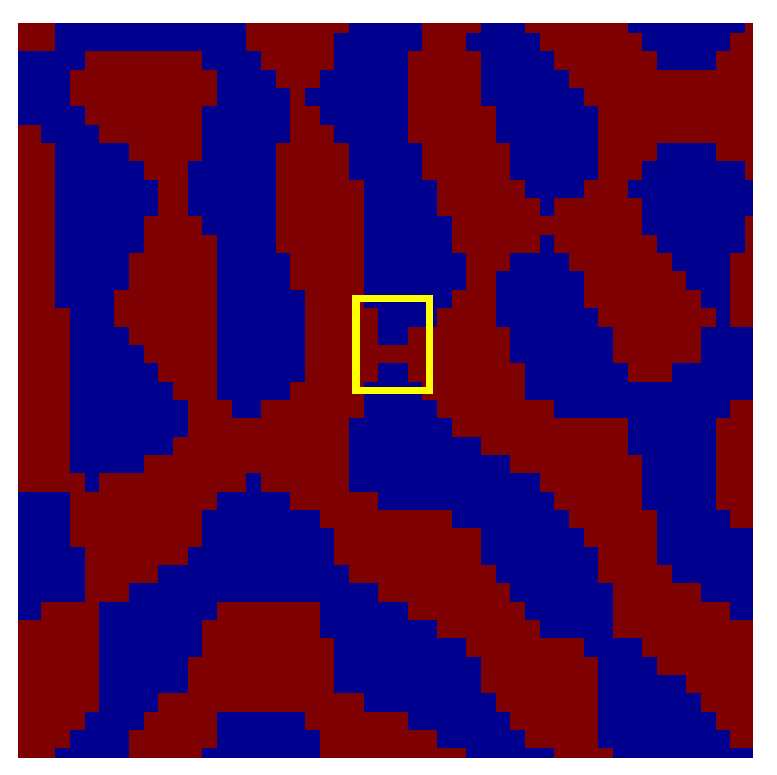
\includegraphics[width=0.49\textwidth]{figs/interpolation/eigenfunction_error_low.eps}
    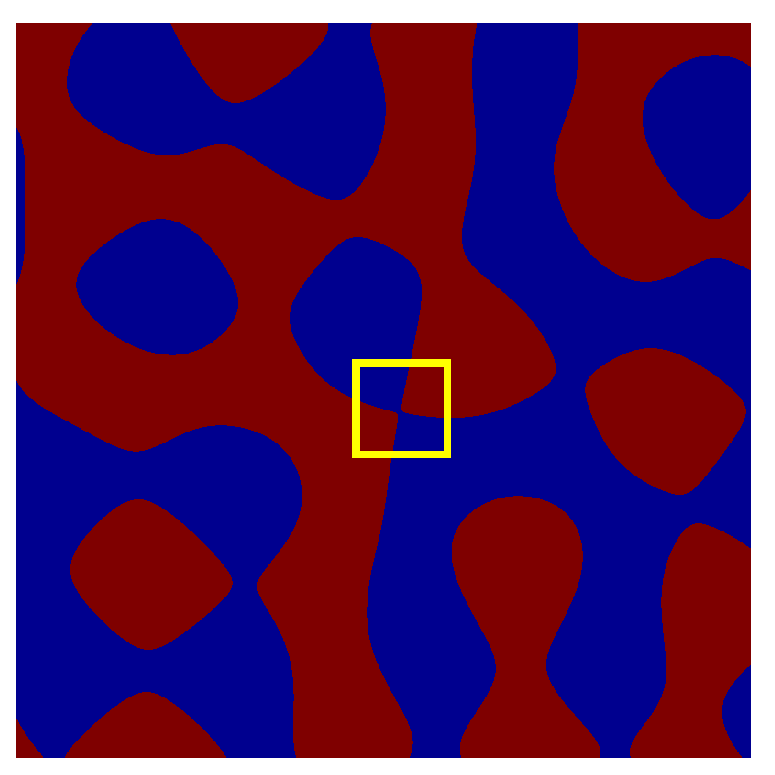
\includegraphics[width=0.49\textwidth]{figs/interpolation/eigenfunction_error_high.eps}
    \caption{An ambiguous nodal domain connection due to coarse sampling. Left: A random plane wave sampled at 10 points per wavelength; right: the same random plane wave sampled at 200 points per wavelength. The ambiguous region at low resolution is highlighted}
    \label{fig:miscounts}
  \end{center}
\end{figure}

We prevent miscounting by interpolating the computed eigenfunction using the functions
\[
J_{n}(k r) \sin(n \theta)
\]
and
\[
J_{n}(k r) \cos(n \theta)
\]
where $J_{n}$ is a regular Bessel function. These functions form a complete basis for solutions of (\ref{eq:helmholtz}) (see appendix \ref{sec:helmholtz_basis}). We fix a value $M$ to be the order of the highest order Bessel function, restricting our basis to the finite set
\begin{equation}
  \label{eq:interp_functions}
  \zeta_{j}(r, \theta)=\begin{cases}
  J_{j}(k r) & \text{if }j=0\\
  J_{j}(k r)\sin(j\theta) & \text{if }1 \le j \le M\\
  J_{j-M}(k r)\cos((j-M)\theta) & \text{if }M+1 \le j \le 2M
  \end{cases}
\end{equation}
We construct a surrogate function
\[
  \tilde{u}(\rr) = \sum_{i=0}^{2M} c_{i} \zeta_{i}(\rr)
\]
as a local approximation to the eigenfunction $u(\rr)$ by fitting the coefficients $c_{i} \in \mathbb{R}$ to minimize the error $\Vert u - \tilde{u} \Vert_{2}$. This function can then be sampled at a higher resolution within the region in question. We define the sampling ratio of this surrogate function to the original eigenfunction to be $\rho$.

\subsection{Triggering Interpolation}
A region is interpolated if and only if, when counting nodal domains, we encounter a point whose sign matches that of a point diagonally adjacent to it, but differs from the signs of the two points adjacent to both it and its diagonal neighbor (fig. \ref{fig:trouble_spot}). In such a case we fill a vector ${\bf v}$ with the eigenfunction values at the stencil points surrounding the four points comprising the ambiguity. We then compute ${\bf w} = P {\bf v}$ where $P$ is the interpolation matrix described above. This vector ${\bf w}$ contains estimated eigenfunction values with a spacing of $\frac{h}{\rho}$ between the four points comprising the ambigious region. We can use these values to determine the connectivity of the nodal domains by traversing pixel-by-pixel from the top-left pixel, in the same manner as above, until we either reach the bottom-right pixel or finish exploring the nodal domain. In the former case the nodal domain containing the top-left pixel connects to the nodal domain containing the bottom-right pixel and in the latter case the nodal domain containing the top-right pixel connects to the nodal domain containing the bottom-left pixel.

\begin{figure}
  \begin{center}
    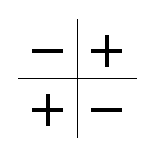
\includegraphics[width=0.2\textwidth]{figs/interpolation/trouble_spot1.eps}
    \hspace{1 cm} 
    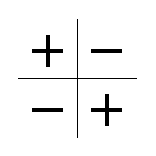
\includegraphics[width=0.2\textwidth]{figs/interpolation/trouble_spot2.eps}
    \caption{Configurations that will result in interpolation}
    \label{fig:trouble_spot}
  \end{center}
\end{figure}

To check the validity of only interpolating at these configurations, we counted nodal domains of $10^{4}$ eigenfunctions that were interpolated everywhere to $\alpha = .023$ and found that mean nodal domains counts agreed within $1\%$. % TODO: get good data

\subsection{Parameter Selection}
\label{sec:params}
Each two pixel by two pixel square defines a region in which interpolation produces upsampled eigenfunction values. The surrogate function however, uses more than just four pixels to fit the coefficients $c_i$. The selection of how many and which surrounding values to use is termed a stencil. Only stencil shapes that are symmetric about the four central points were considered. The four shapes considered are shown in figure \ref{fig:stencils}. The most important consideration in choosing a stencil was the accuracy of the interpolation. The size of the stencil affects the computational cost of interpolation but this difference is trivial.

\begin{figure}
  \begin{center}
    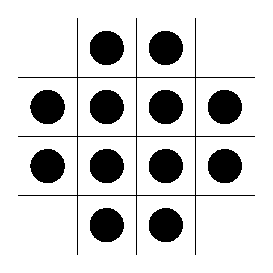
\includegraphics[width=0.2\textwidth]{figs/stencils/4x4_no_corners_centered.eps}
    \hspace{1.5 cm}
    
\includegraphics[width=0.2\textwidth]{figs/stencils/4x4_centered.eps}
    \linebreak
    \linebreak
    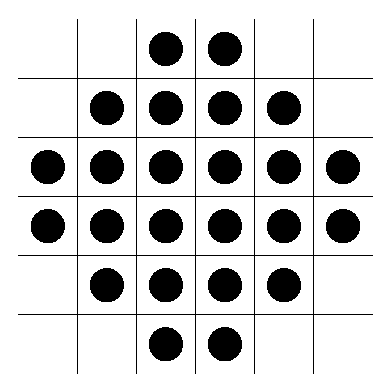
\includegraphics[width=0.3\textwidth]{figs/stencils/4x4+2_centered.eps}
    \hspace{0.4 cm}
    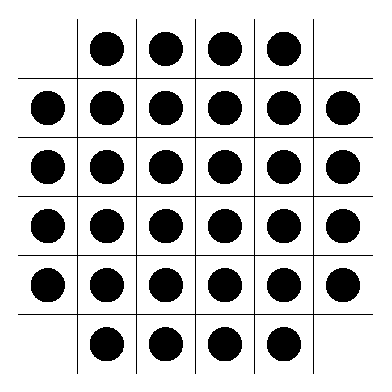
\includegraphics[width=0.3\textwidth]{figs/stencils/6x6_no_corners_centered.eps}
    \caption{The four stencil shapes considered for interpolation}
    \label{fig:stencils}
  \end{center}
\end{figure}

The accuracy of interpolation also depends on $M$ and $\alpha = k h$, which must be considered simultaneously with the choice of stencil. Figure \ref{fig:errors_all} shows a comparison of the infinity norm of the interpolation error over various values of $M$ and $\alpha$ for each of the stencils shown above.

\begin{figure}
  \begin{center}
    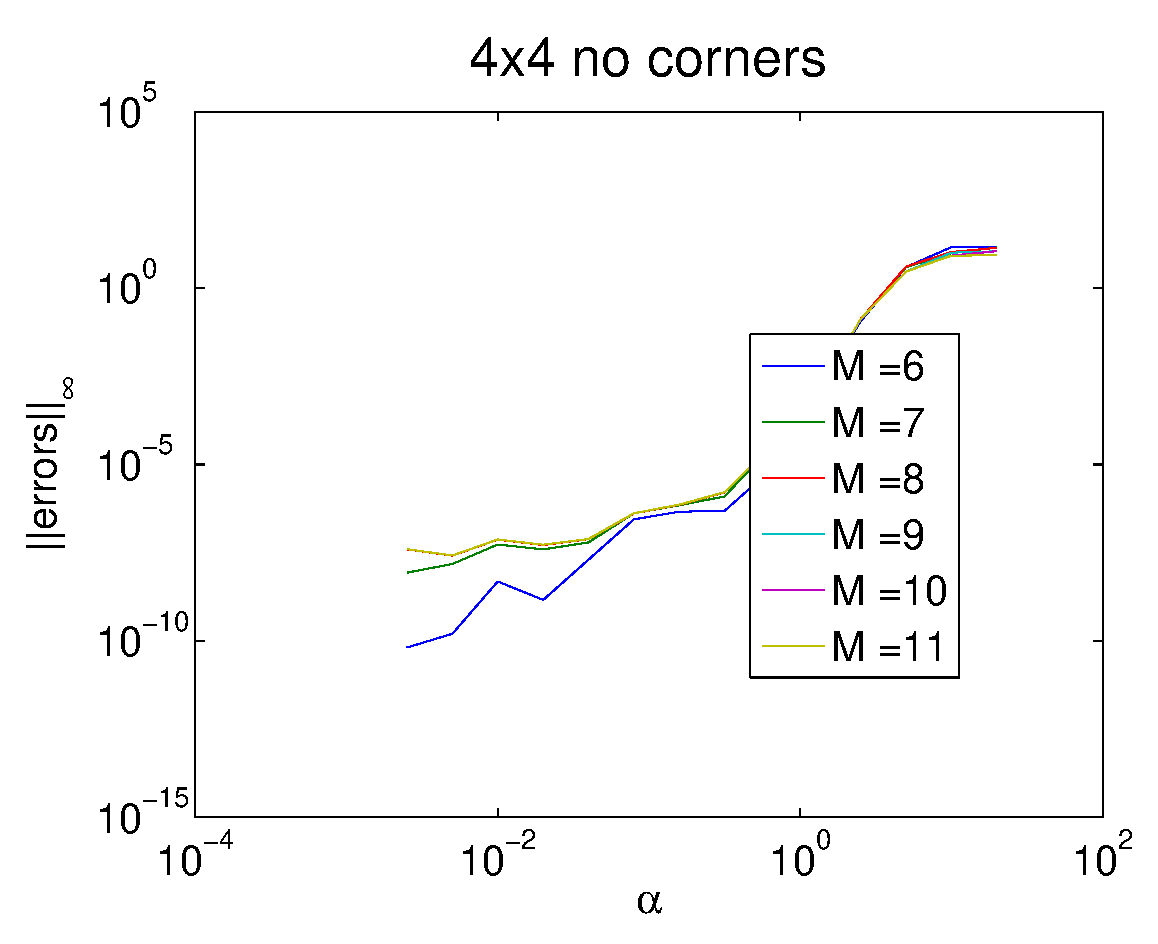
\includegraphics[width=0.8\textwidth]{figs/interpolation/error_norms_1.eps}
    \linebreak
    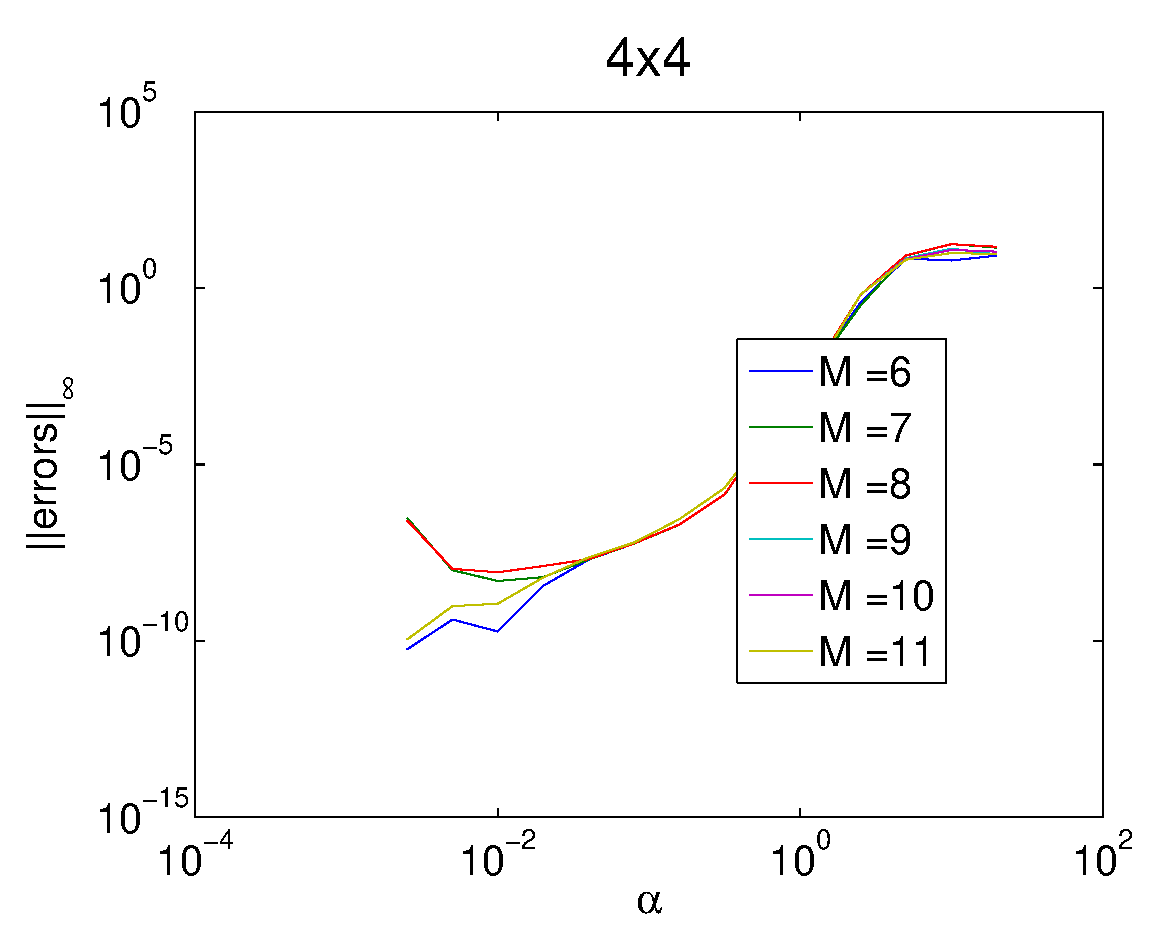
\includegraphics[width=0.8\textwidth]{figs/interpolation/error_norms_2.eps}
    \caption{Comparison of interpolation error norms over $M$ and $\alpha$ for each stencil.}
    \label{fig:errors_all}
  \end{center}
\end{figure}

\begin{figure}
  \begin{center}
    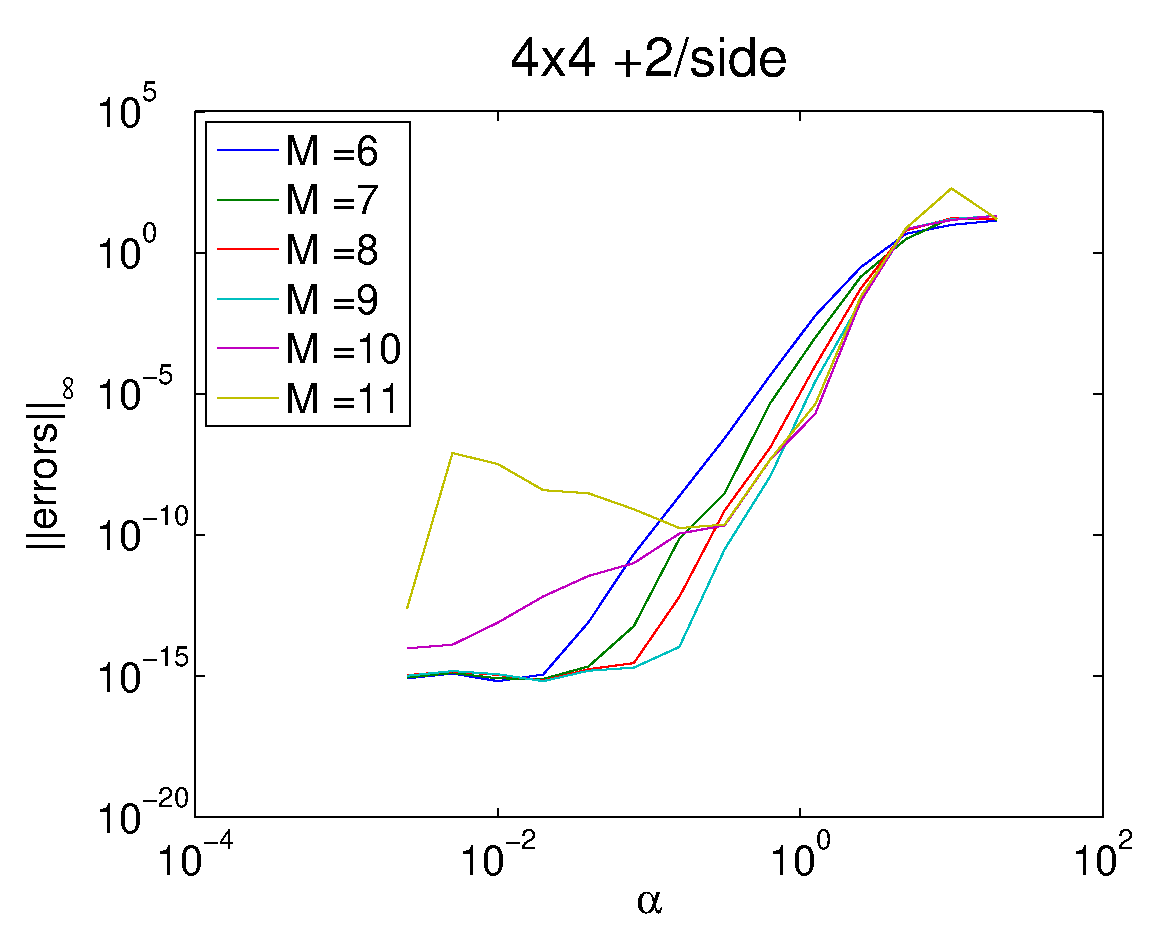
\includegraphics[width=0.8\textwidth]{figs/interpolation/error_norms_3.eps}
    \linebreak
    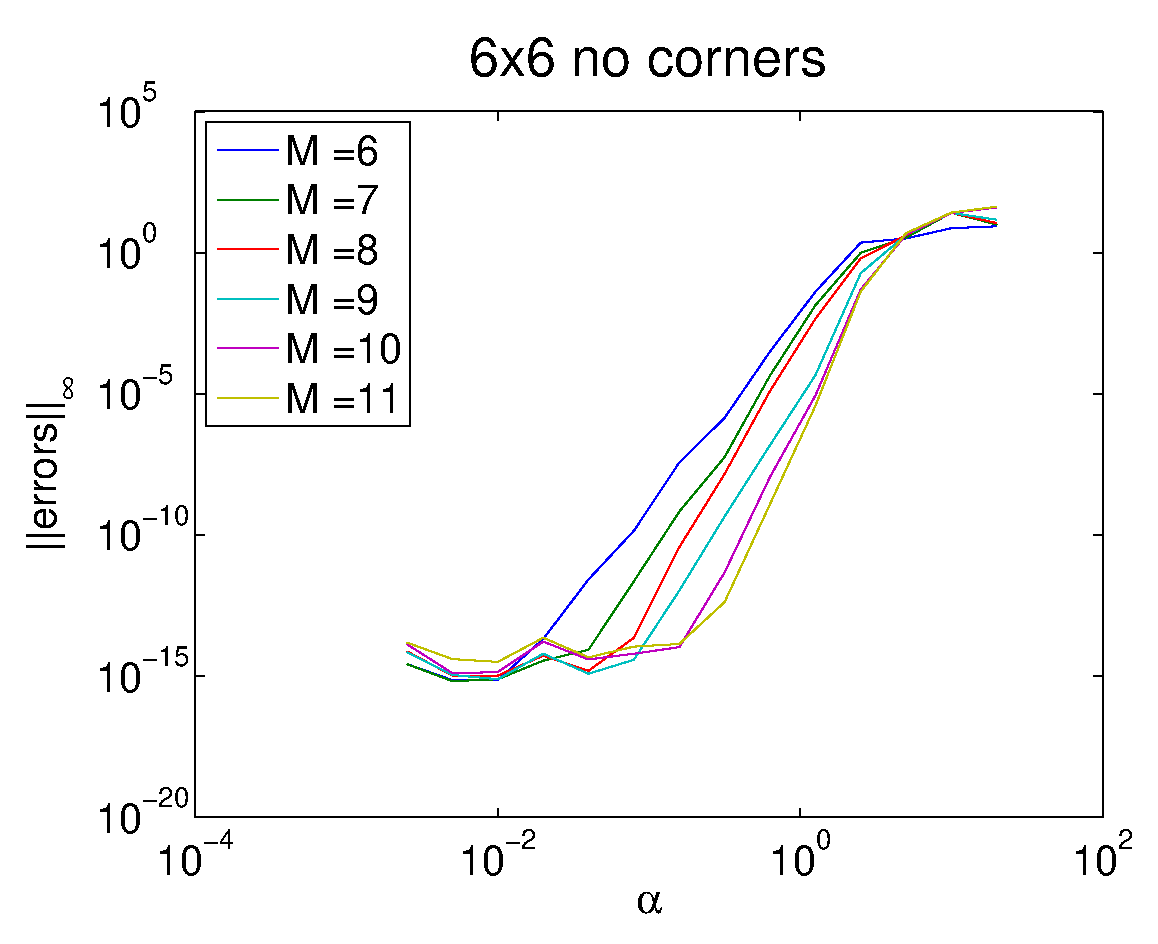
\includegraphics[width=0.8\textwidth]{figs/interpolation/error_norms_4.eps}
  \end{center}
\end{figure}

Based on these data, we chose to use the 24-point stencil with $M=9$ and $\alpha \in [0.5, 0.7]$ for interpolation. For this choice of parameters we expect errors in interpolated eigenfunction values of order $10^{-6}$. We use an upsampling ratio of $\rho = 30$, which we have found to be sufficient to resolve ambiguities in nearly all cases.

\subsection{Numerical Implementation}
We construct a matrix to transform values on a stencil to interpolated values in the center of the stencil, performing the process described above with a single matrix multiplication. We construct the interpolation matrix as
\[
P = H L^{+}
\]
Where $L$ is an $S$ by $2M+1$ matrix (where $S$ is the number of stencil points) which contains evaluations of Bessel functions at stencil points, $H$ is a $(\rho + 1)^{2}$ by $2M+1$ contains evaluations of Bessel functions at high resolution and $^{+}$ denotes the pseudoinverse. Specifically,
\[
L_{ij} =\begin{cases}
J_{j}(r_{i}) & \text{for } j = 0 \text{ and } 0 \le i < T\\
J_{j}(r_{i}) \sin{(j \theta_{i})} & \text{for } 1 \le j \le M \text{ and } 0 \le i < T\\
J_{j-M}(r_{i}) \cos{((j-M) \theta_{i})} & \text{for } M+1 \le j \le 2M+1 \text{ and } 0 \le i < T
\end{cases}
\]
and
\[
H_{ij} =\begin{cases}
J_{j}(\tilde{r}_{i}) & \text{for } j = 0 \text{ and } 0 \le i < \gamma\\
J_{j}(\tilde{r}_{i}) \sin{(j \tilde{\theta}_{i})} & \text{for } 1 \le j \le M \text{ and } 0 \le i < \gamma\\
J_{j-M}(\tilde{r}_{i}) \cos{((j-M) \tilde{\theta}_{i})} & \text{for } M+1 \le j \le 2M+1 \text{ and } 0 \le i < \gamma
\end{cases}
\]
where $T$ is the number of points in the stencil, $\gamma = (\rho + 1)^{2}$ and $(r_{i},\theta_{i})$ and $(\tilde{r}_{i},\tilde{\theta}_{i})$ are points in the stencil and inner square, respectively, expressed in polar coordinates.

$P$ acts on a vector of eigenfunction values in a stencil and produces interpolated values in the center square of the stencil (fig. \ref{fig:upsample_action}).

\begin{figure}
  \begin{center}
    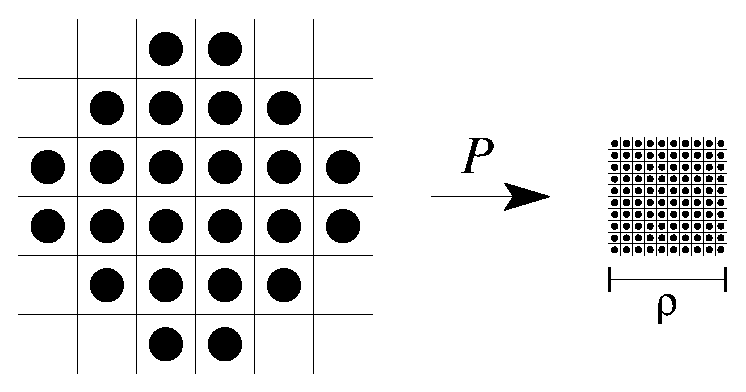
\includegraphics[width=\textwidth]{figs/stencils/upsample_action.eps}
    \caption{Visualization of the action of $P$ as a mapping. $P$ maps eigenfunction values on a coarse grid to eigenfunction values on a fine grid.}
    \label{fig:upsample_action}
  \end{center}
\end{figure}

The pseudoinverse $L^{+}$ is computed using a singular value decomposition as follows,
\[
L^{+} = V \Sigma^{+} U^{*}
\]
where $L = U^{*} \Sigma V$ is a singular value decomposition of $L$ and $\Sigma$ is a diagonal matrix of singular values with
\[
\Sigma^{+}_{ii} =\begin{cases}
\Sigma_{ii}^{-1} & \text{if }\Sigma_{ii} > \epsilon\\
\Sigma_{ii} & \text{otherwise}
\end{cases}
\]
where $\epsilon = \gamma \epsilon_{double} \Sigma_{11}$ where $\epsilon_{double} = 1.11e{-16}$ is the difference between one and the smallest IEEE double precision floating point number greater than one. Singular values less than $\epsilon$ are considered to be zero within working precision.


\section{Analysis}

\subsection{Probability of ambiguous region}
Here we derive an upper bound on the probability of a trouble region using random plane waves \ref{eq:rpw}. Applying the Jacobi-Anger expansion \cite{abramowitz}
\[
\exp(\mathrm{i} k r \cos \theta) = \sum_{l \in \mathbb{Z}} \mathrm{i}^{l} \exp{\left\{\mathrm{i} l \theta \right\}} J_{l}(kr)
\]
and the fact that $\hat{n}_{n} \cdot \rr = r \cos{ \left( \theta - \frac{2 \pi n}{N} \right) }$ produces
\begin{equation}
  \label{eq:rpw_bessel_expansion}
  u(\rr) = \Re \left[ \sum_{l \in \mathbb{Z}} \mathrm{i}^{l} \tilde{\omega}_{l} \exp{\left\{\mathrm{i} l \theta \right\}} J_{l}(kr) \right]
\end{equation}
where $\rr = (r, \theta)$ in polar coordinates and $\tilde{\omega}_{l}$ are given by
\[
\tilde{\omega}_{l} = \lim_{N \rightarrow \infty} \frac{1}{\sqrt{N}} \sum_{n=1}^{N} \omega_{n} \mathrm{i}^{l} \exp{\left\{-\mathrm{i} l \frac{2 \pi n}{N} \right\}}
\]
Fixing $N$, we can express the transformation which takes $\overrightarrow{\omega}$ to $\overrightarrow{\tilde{\omega}}$ (as vectors) as a matrix
\[
\overrightarrow{\tilde{\omega}}^{(N)} = A^{(N)} \overrightarrow{\omega}^{(N)}
\]
where entries of $A^{(N)}$ are given by
\[
a_{mn} = \frac{1}{\sqrt{N}} \mathrm{i}^{m} \exp{\left\{-\mathrm{i} m \frac{2 \pi n}{N} \right\}} = \frac{1}{\sqrt{N}} \exp{\left\{-\mathrm{i} m \left(\frac{2 \pi n}{N} - \frac{\pi}{2}\right) \right\}} 
\]
The operator $A$ is simply a discrete Fourier transform and therefore acts on $\omega_{n} \sim \mathcal{N}(0,1)$ i.i.d. to produce $\tilde{\omega}_{n} \sim \mathcal{N}(0, 1)$ i.i.d.

Expanding the first three terms of \ref{eq:rpw_bessel_expansion} gives
\[
u(\rr) = a_{0} J_{0}(kr) + J_{1}(kr) (a_{1} \cos{\theta} + b_{1} \sin{\theta}) + J_{2}(kr) (a_{2} \cos{2 \theta} + b_{2} \sin{2 \theta}) + \ldots
\]
where $a_{0} = \Re \left[ \tilde{\omega}_{0} \right]$, $a_{1,2} = \Re \left[ \tilde{\omega}_{1} - \tilde{\omega}_{-1} \right]$, and $b_{1,2} = \Im \left[ \tilde{\omega}_{1} - \tilde{\omega}_{-1} \right]$. Note that $a_{0} \sim \mathcal{N}(0,1)$ and $a_{1}, b_{1}, a_{2} \sim \mathcal{N}(0,\sqrt{2})$.

\begin{figure}
  \begin{center}
    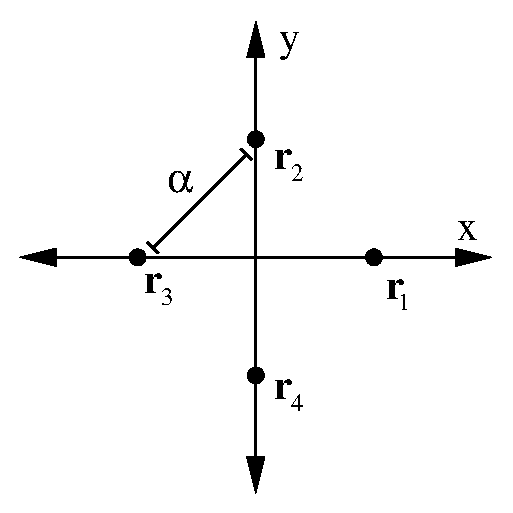
\includegraphics[width=0.5\textwidth]{figs/interpolation/four_points_on_axes.eps}
    \caption{Four evaluation points in coordinate system}
    \label{fig:four_points}
  \end{center}
\end{figure}

We now consider four points forming a square of side length $\alpha$. We define a coordinate system with origin at the center of the square and axes rotated such that each corner of the square falls on either the $x$- or $y$-axis (figure \ref{fig:four_points}). We label the four points $\rr_{1}$ through $\rr_{4}$. Evaluating the three term expansion of $u(\rr)$ at the four points gives
\begin{align*}
  u(\rr_{1}) & = a_{0} \beta_{0} + a_{1} \beta_{1} + a_{2} \beta_{2} \\
  u(\rr_{2}) & = a_{0} \beta_{0} + b_{1} \beta_{1} - a_{2} \beta_{2} \\
  u(\rr_{3}) & = a_{0} \beta_{0} - a_{1} \beta_{1} + a_{2} \beta_{2} \\
  u(\rr_{4}) & = a_{0} \beta_{0} - b_{1} \beta_{1} - a_{2} \beta_{2}
\end{align*}
where $\beta_{i} = J_{i} \left( k \frac{\alpha}{\sqrt{2}} \right)$. Interpolation is required if $u(\rr_{1}), u(\rr_{3}) < 0$ and $u(\rr_{2}), u(\rr_{4}) > 0$ (or the reverse case) which gives the system of inequalities
\begin{align*}
  a_{0} \beta_{0} + a_{1} \beta_{1} + a_{2} \beta_{2} & < 0 \\
  a_{0} \beta_{0} + b_{1} \beta_{1} - a_{2} \beta_{2} & > 0 \\
  a_{0} \beta_{0} - a_{1} \beta_{1} + a_{2} \beta_{2} & < 0 \\
  a_{0} \beta_{0} - b_{1} \beta_{1} - a_{2} \beta_{2} & > 0
\end{align*}
which is equivalent to
\begin{align*}
  a_{2} & < 0 \\
  a_{0} & < a_{2} \frac{\beta_{2}}{\beta_{0}} \\
  a_{1} & < a_{2} \frac{2 \beta_{2}}{\beta_{1}} \\
  b_{1} & < 0
\end{align*}
Thus the probability of a configuration of four points requiring interpolation is given by
\begin{equation}
  2 \int_{-\infty}^{0} \int_{-\infty}^{0} \int_{-\infty}^{a_{2} \frac{\beta_{2}}{\beta_{0}}} \int_{-\infty}^{a_{2} \frac{2 \beta_{2}}{\beta_{1}}} f(a_{0}, a_{1}, b_{1}, a_{2}) \ud a_{1} \ud a_{0} \ud b_{1} \ud a_{2}
\end{equation}
where the factor of two is inserted to account for the possibility of the inequalities being reversed and $f(a_{0}, a_{1}, b_{1}, a_{2})$ is a four dimensional Gaussian distribution
\[
f(a_{0}, a_{1}, a_{2}) = \frac{1}{(2 \pi)^{2} {\vert \Sigma \vert}^{\frac{1}{2}}} \exp{\left\{ {\bf a}^{T} \Sigma^{-1} {\bf a} \right\}}
\]
where
\[
{\bf a} = \left(
\begin{array}{c}
  a_{0} \\
  a_{1} \\
  b_{1} \\
  a_{2}
\end{array}
\right)
\hspace{1 cm}
\Sigma = \begin{pmatrix}
  1 & 0 & 0 & 0 \\
  0 & 2 & 0 & 0 \\
  0 & 0 & 2 & 0 \\
  0 & 0 & 0 & 2
\end{pmatrix}
\]
applying the linear transformation
\begin{align*}
  x_{1} = & a_{0} \\
  x_{2} = & a_{0} - \frac{\beta_{2}}{\beta_{0}} a_{2} \\
  x_{3} = & a_{1} - \frac{2 \beta_{2}}{\beta_{1}} a_{2} \\
  x_{4} = & b_{1}
\end{align*}
produces the integral
\begin{equation}
  \label{eq:theoretical_ambiguity_prob}
  2 \int_{-\infty}^{0} \int_{-\infty}^{0} \int_{-\infty}^{0} \int_{-\infty}^{0} f_{X}(x_{0}, x_{1}, x_{2}, x_{3}) \ud{x_{3}} \ud{x_{2}} \ud{x_{1}} \ud{x_{0}}
\end{equation}
where
\[
f_{X}(x_{0}, x_{1}, x_{2}, x_{3}) = \frac{1}{(2 \pi)^{2} {\vert (J \Sigma J^{T})^{-1} \vert}^{\frac{1}{2}}} \exp{\left\{ \xx^{T} J \Sigma J^{T} \xx \right\}}
\]
is the Gaussian distribution $f$ under the linear transformation and $J$ is the Jacobian of this transformation
\[
J = \begin{pmatrix}
  1 & 0 & 0 & 0 \\
  1 & 0 & 0 & -\frac{\beta_{2}}{\beta_{0}} \\ 
  0 & 1 & 0 & \frac{2 \beta_{2}}{\beta_{1}} \\
  0 & 0 & 1 & 0
\end{pmatrix}
\]
This integral can be computed numerically; figure \ref{fig:theoretical_ambiguity_prob} shows the probability of such an error occuring at a randomly chosen two pixel by two pixel square. These results appear to match empirical measures of interpolations per pixel to within a constant factor of approximately $2.5$. %TODO: get good data

\begin{figure}
  \begin{center}
  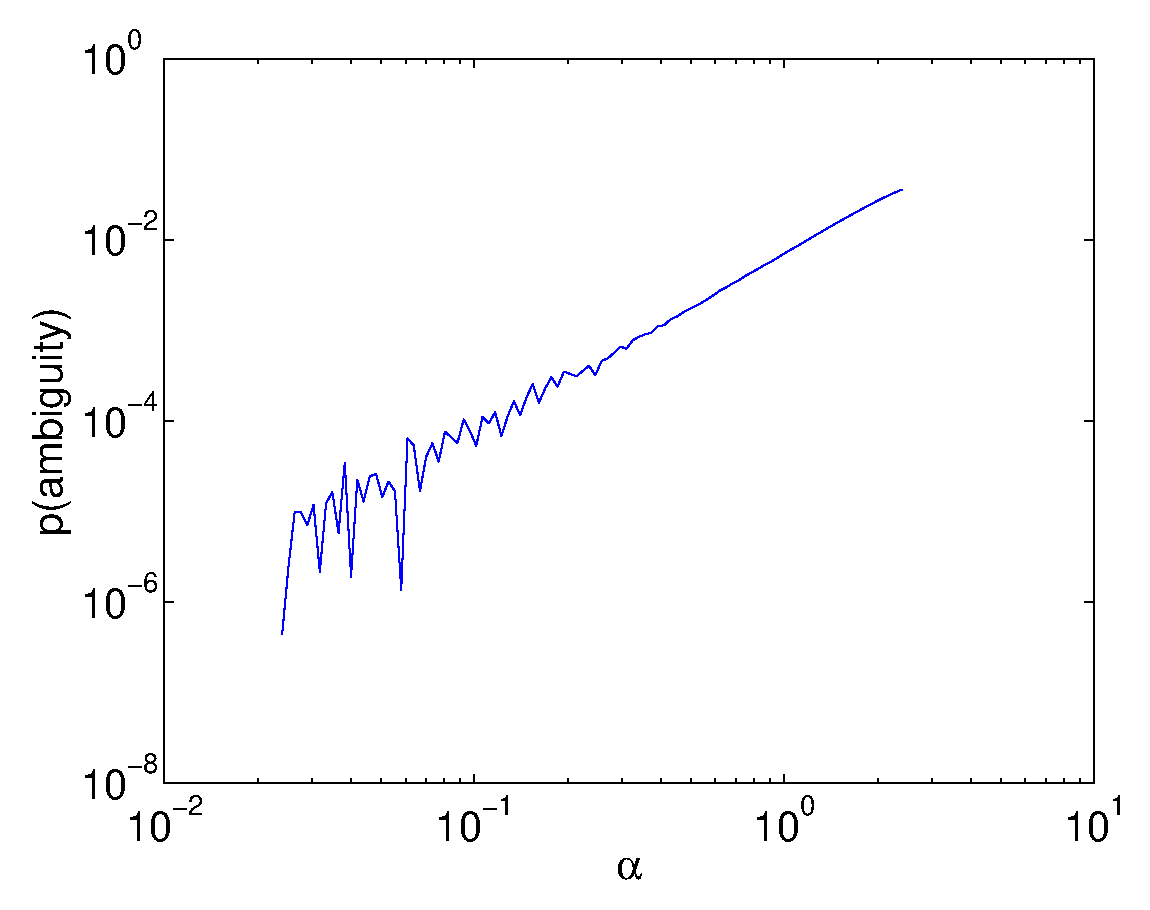
\includegraphics[width=\textwidth]{figs/interpolation/theoretical_ambiguity_prob.eps}
  \caption{Theoretical probability of an ambiguity when sampling at $\alpha$ by \ref{eq:theoretical_ambiguity_prob}. Small values of alpha produce highly correlated variables in the transformed coordinate system, which produce numerical instabilities in the integration of the Gaussian.}
  \label{fig:theoretical_ambiguity_prob}
  \end{center}
\end{figure}

The heuristic we use when deciding where to interpolate misses some very rare cases where domains connect between sampled points. See \cite{mischaikow} for a more complete characterization of sampling errors when computing nodal domains in two dimensions.

\section{Counting Nodal Domains}
\label{sec:counting}
Eigenfunctions are sampled on a regular grid with dimension $n_{y}$ by $n_{x}$; each point in this grid will be referred to as a ``pixel.'' Nodal domains are counted by exploring domains pixel-by-pixel, marking each pixel as ``counted'' in an $n_{y}$ by $n_{x}$ bit array once it has been seen. The searching algorithm used to explore each domain is a hybrid depth- and breadth-first method where for each pixel, the sign of each uncounted neighboring pixel is compared to the sign of the nodal domain and if the sign matches, the neighboring pixel is pushed onto a stack. Exploration then continues by popping a pixel off of the stack.

This hybrid method was chosen because it requires fewer comparisons than a depth-first search (where a pixel may be popped from the stack up to four times, once for each neighbor, versus only once in this method) and allows an efficient stack implementation using a dynamically sized array, whereas a breadth-first search requires a queue, which cannot be implemented as efficiently as a stack. A linked-list implementation of a stack or queue was found to add approximately $15\%$ runtime overhead due to frequent memory allocations. An array implementation of a queue can be accomplished by treating the array as circular but this requires additional comparisons when enqueueing and dequeueing as compared to an array implementation of a stack.

\begin{algorithm}
  \caption{Nodal domain counting algorithm}
  \begin{algorithmic}
    \Require $grid$ is $ny$ by $nx$ matrix containing eigenfunction values on billiard
    \Require $\alpha = k h$, $M$ is highest order Bessel function to interpolate with, $\rho$ is ratio to interpolate by
    \Require $counted$ is $ny$ by $nx$ and $counted[i][j] = UNCOUNTED$ if the point at $i,j$ is in $\Omega$, else $counted[i][j] = COUNTED$

    \item[]
    \Function{CountNodalDomains}{$grid, counted, \alpha, M, \rho$}
        \State $interp \gets CreateInterpMatrix(\alpha, M, \rho)$
        \State $i,j,domains \gets 0$
        \While{$i, j \gets FindNextUnseen(counted, i, j)$}
            \State $domains \gets domains + 1$
            \State $FindDomain(grid, counted, i, j, domain\_num, interp)$
        \EndWhile \\
        \Return $domains$
    \EndFunction

    \item[]
    \Function{FindNextUnseen}{$counted, y, x$}
        \For{$i \in y \ldots ny$}
            \For{$j \in 1\ldots nx$}
                \If{$i=y$ and $j \leq x$}
                    \State continue
                \EndIf
                \If{$counted[i][j] = UNCOUNTED$}
                    \State \Return $i,j$
                \EndIf
            \EndFor
        \EndFor
        \State \Return $NULL$
    \EndFunction
    \algstore{count}
  \end{algorithmic}
\end{algorithm}

\clearpage
\begin{algorithm}
  \ContinuedFloat
  \caption{Nodal domain counting algorithm (continued)}
  \begin{algorithmic}
    \algrestore{count}

    \Function{FindDomain}{$grid, counted, i, j, interp$}
        \State $left, above, right, below \gets FALSE$, 
        \State $s.push(j,i)$
        \State $counted[i][j] = COUNTED$
        \State $sign \gets sign(grid[i][j])$
        \Comment $s$ is a stack
        \While{$x,y \gets s.pop()$}
            \If{$InGrid(x-1,y)$}
                \If{$sign(grid[y][x-1]) = sign$}
                    \State $left \gets TRUE$
                    \If{$counted[x-1][y] = UNCOUNTED$}
                        \State $counted[y][x-1] = COUNTED$
                        \State $s.push(x-1,y)$
                    \EndIf
                \EndIf
            \EndIf
            \State $\ldots$ \Comment Same for $above$, $right$, and $below$
            \If{$InGrid(x-1,y-1)$ and $above$ and $left$}
                \If{$sign(grid(x-1,y-1)) = sign$}
                  \If{not $IsInterpolated(counted, x-1,y-1)$}
                      \State $Interpolate(grid, counted, x-1, y-1, interp)$
                  \EndIf
                  \If{$ConnectedAboveLeft(counted,x,y)$}
                      $s.push(x-1,y-1)$
                  \EndIf
                \EndIf
            \EndIf
            \State $\ldots$ \Comment Same for $below$ and $left$, $below$ and $right$, and $above$ and $right$
        \EndWhile
    \EndFunction
  \end{algorithmic}
\end{algorithm}

This algorithm has runtime $O(N)$. This is because the method performs a constant number of comparisons for each pixel in the eigenfunction plus $O(N)$ total comparisons searching for an unseen pixel after a nodal domain has been explored. Interpolation occurs $O(N)$ times and each matrix-vector multiply takes constant time because the number of stencil points $S$ and the upsampling ratio $\rho$ are constant.

This algorithm requires $O(N)$ space for the array $counted$ which we use to store for each pixel, whether it is in the domain, has been counted already, and has been interpolated. In addition, this method uses a dynamically sized array as a stack whose size is (loosely) bounded above by the number of pixels in the nodal domain being explored.

\chapter{Results}

\section{Data Collected}
We computed approximately $10^{5}$ eigenfunctions amounting to over $800$ GB of data and counted $1.5$ billion nodal domains. This data required approximately $8000$ CPU hours, running on a cluster with about $30$ cores.

\subsection{Run time}
For both billiards considered here $B \sim k$. Thus, in practice $N \gg n$ and $N \gg B$ so it is primarily $N$ (which scales like $\alpha^{-2}$) that determines the time to compute eigenfunctions. Computation time is dominated by eigenfunction evaluation, which is dominated by basis function evaluations (fig. \ref{fig:timing}).

\begin{figure}
  \begin{center}
    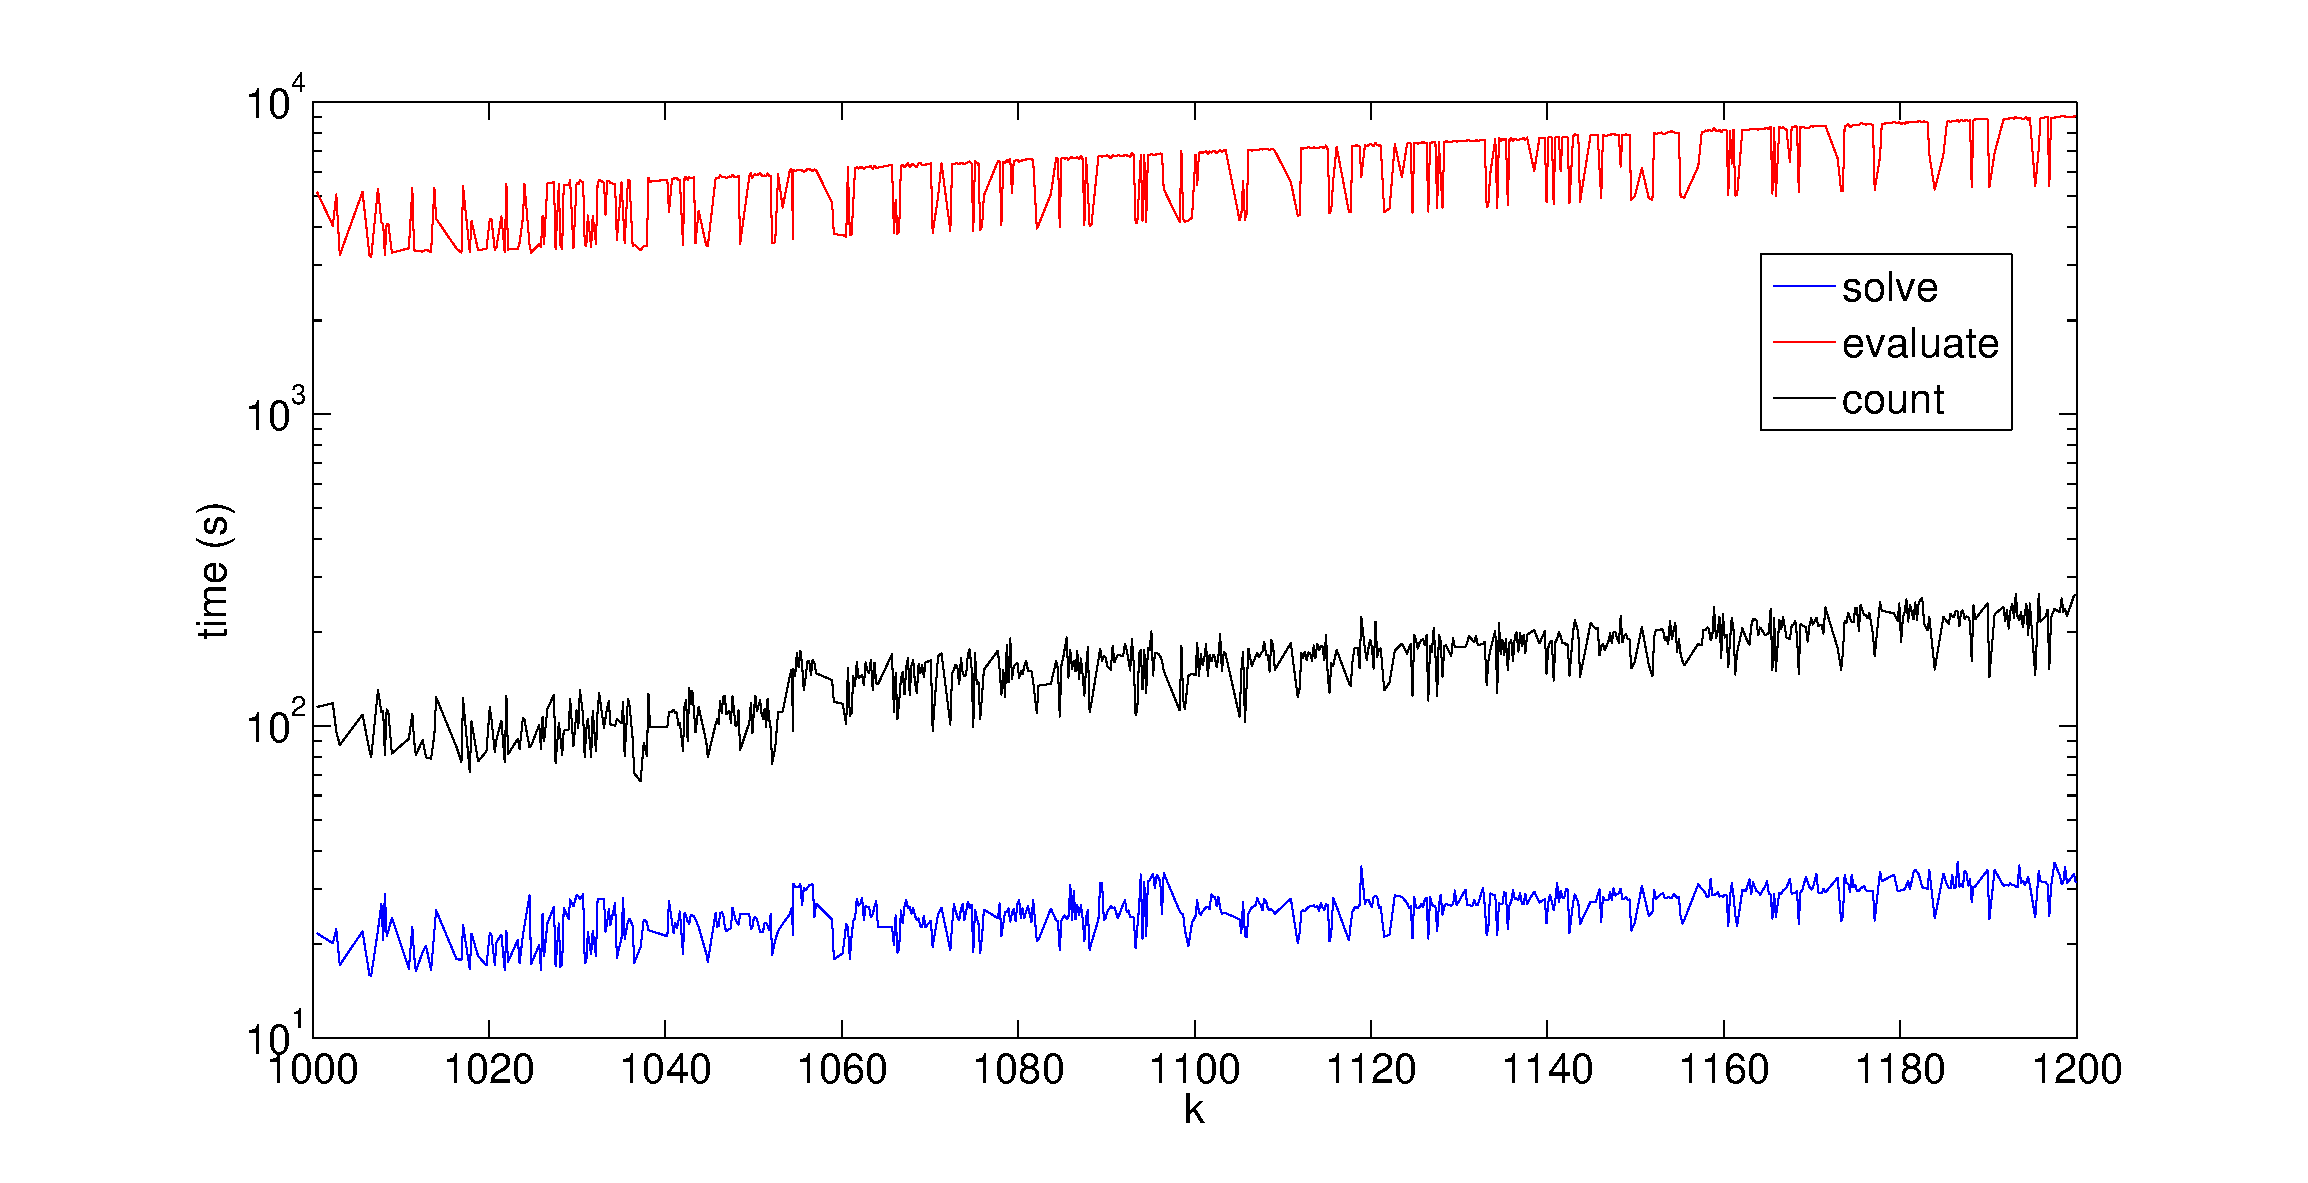
\includegraphics[width=\textwidth]{figs/timing/timing_comp_1000_to_1200.eps}
    \caption{Comparison of run times at $\alpha = 0.5$ of solving for basis coefficients, evaluating eigenfunctions, and counting nodal domains. Evaluating eigenfunctions dominates runtime, taking approximately 97\% of computation time.}
    \label{fig:timing}
  \end{center}
\end{figure}

\subsection{Prior Work}
Bogomolny and Schmit \cite{bogomolny07} have conducted a small numerical study of their conjectures but investigated only the stadium billiard and collected only a few hundred eigenfunctions. These eigenfunctions were collected around $k=100$ which we have shown is far from the asymptotic regime (fig. \ref{fig:mean}). Keating, Marklof and Williams \cite{keating} have performed a related study on quantum maps, for which they verified all three conjectures of Bogomolny and Schmit, using a few thousand eigenstates (which are much less costly to compute for quantum maps as compared to quantum billiards).

\section{Mean of number of nodal domains}
We find that the scaled mean number of nodal domains for the Sinai billiard converges to $0.0596 \pm 1.724e{-5}$, which is $4.61\%$ below the value of conjecture \ref{conj:mean}. This result represents a deviation of $167 \sigma$ and is therefore very statistically significant.

Nodal counts in the stadium billiard approached scaled mean of $0.0535 \pm 3.991e{-5}$, which is $14.36\%$ below the conjectured value and a deviation of $225 \sigma$.

We find that the mean for random plane waves also disagrees with the conjectured value and in fact converges $.0589 \pm 1.42e{-4}$, which very nearly matches the asymptotic mean of the Sinai billiard. This indicates that the percolation model is not an accurate model of quantum chaos.

The mean number of the nodal domains of the percolation model agrees well with the conjectured value. These were computed on a unit grid as described in \ref{sec:percolation}.

In all models, we find a relatively slow convergence toward the asymptotic mean. Bogomolny and Schmit \cite{bogomolny} predict a convergence of the form $A + B/k$, which we fit to data to predict asymptotic values. We find fitted values of $B$ between $3$ and $5$ for the various billiards and models considered, indicating that it is necesarry to approach $k ~ 10^{3}$ to obtain counts within $~5\%$ of the asymptotic value.

\begin{figure}
  \begin{center}
    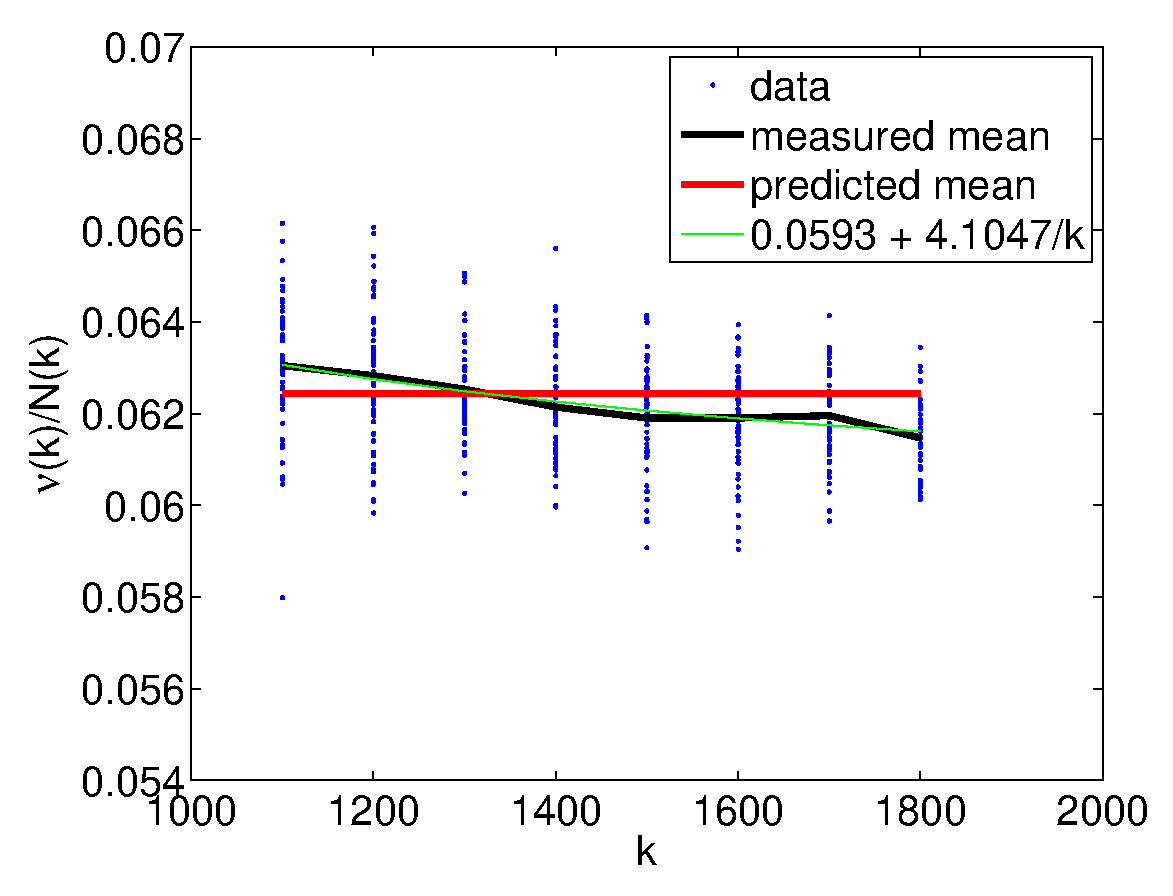
\includegraphics[width=0.9\textwidth]{figs/results/qugrs_all_mean.eps}
    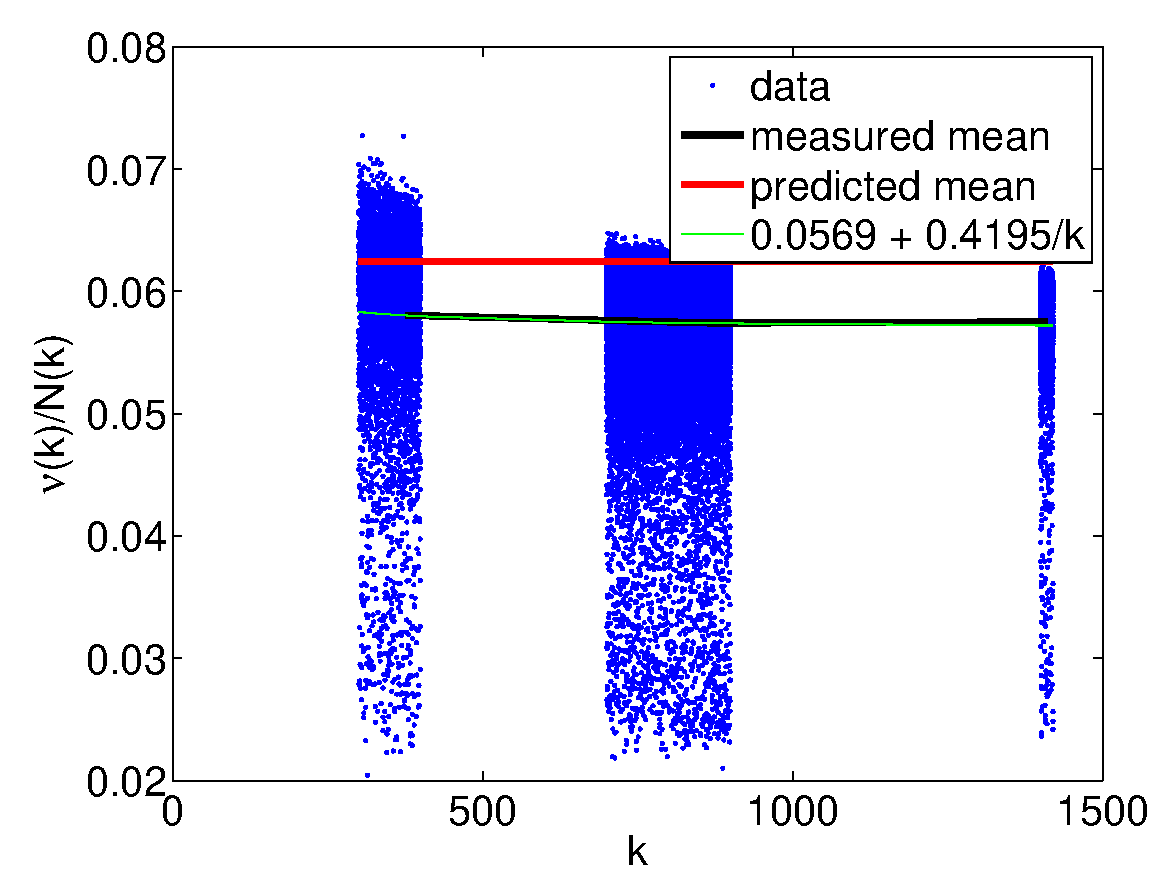
\includegraphics[width=0.9\textwidth]{figs/results/qust_all_mean.eps}
    \caption{Mean number of nodal domains. Above: Sinai; below: stadium. The least-squares best fit of the form $A + B/k$ is shown in green.}
    \label{fig:mean}
  \end{center}
\end{figure}

\begin{figure}
  \begin{center}
    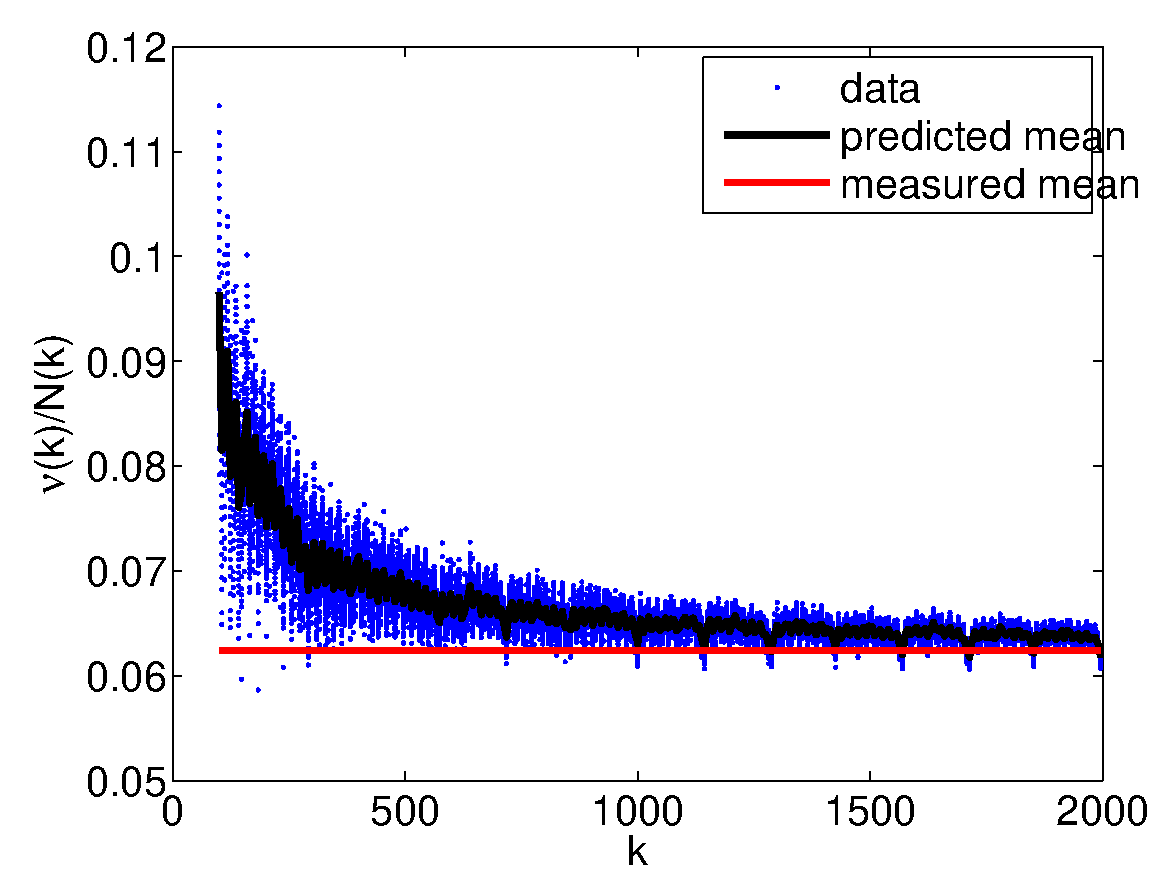
\includegraphics[width=0.9\textwidth]{figs/results/perc_100_to_2000_mean.eps}
    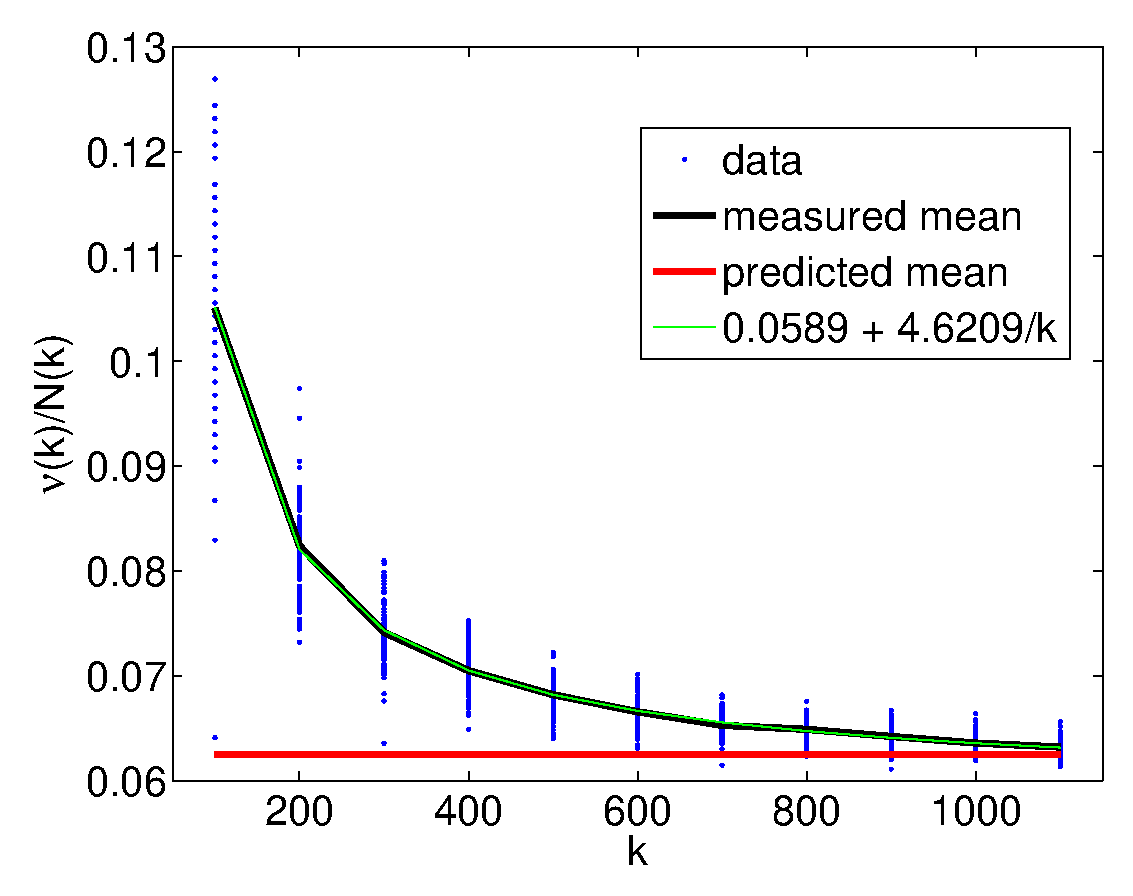
\includegraphics[width=0.9\textwidth]{figs/results/rpw_all_mean.eps}
    \caption{Mean number of nodal domains. Above: percolation with $k \in \{100, 106, 112, \ldots, 1998\}$; below: random plane waves with $k \in \{100, 200, \ldots, 1100\}$ with 100 repetitions at each $k$.}
  \end{center}
\end{figure}

\section{Variance of number of nodal domains}
The variance of number of nodal domains in quantum chaotic eigenfunctions does not agree with conjecture \ref{conj:variance} for either billiard shape (fig. \ref{fig:variance}). The quarter generalized rectangular Sinai billiard has a variance of scaled nodal domains counts of $0.107$, which is $2.13$ times the value of conjecture \ref{conj:variance}. The quarter stadium has a variance of scaled nodal domain counts of $2.70$, which is over $50$ times the conjectured value.

The random plane wave model has a variance of scaled nodal domain counts of $0.0883$, which is again comparable to the Sinai value. The percolation model has a variance of $0.0501$, which agrees well with the predicted value, having a relative error of $2.40e{-3}$.

\begin{figure}
  \begin{center}
    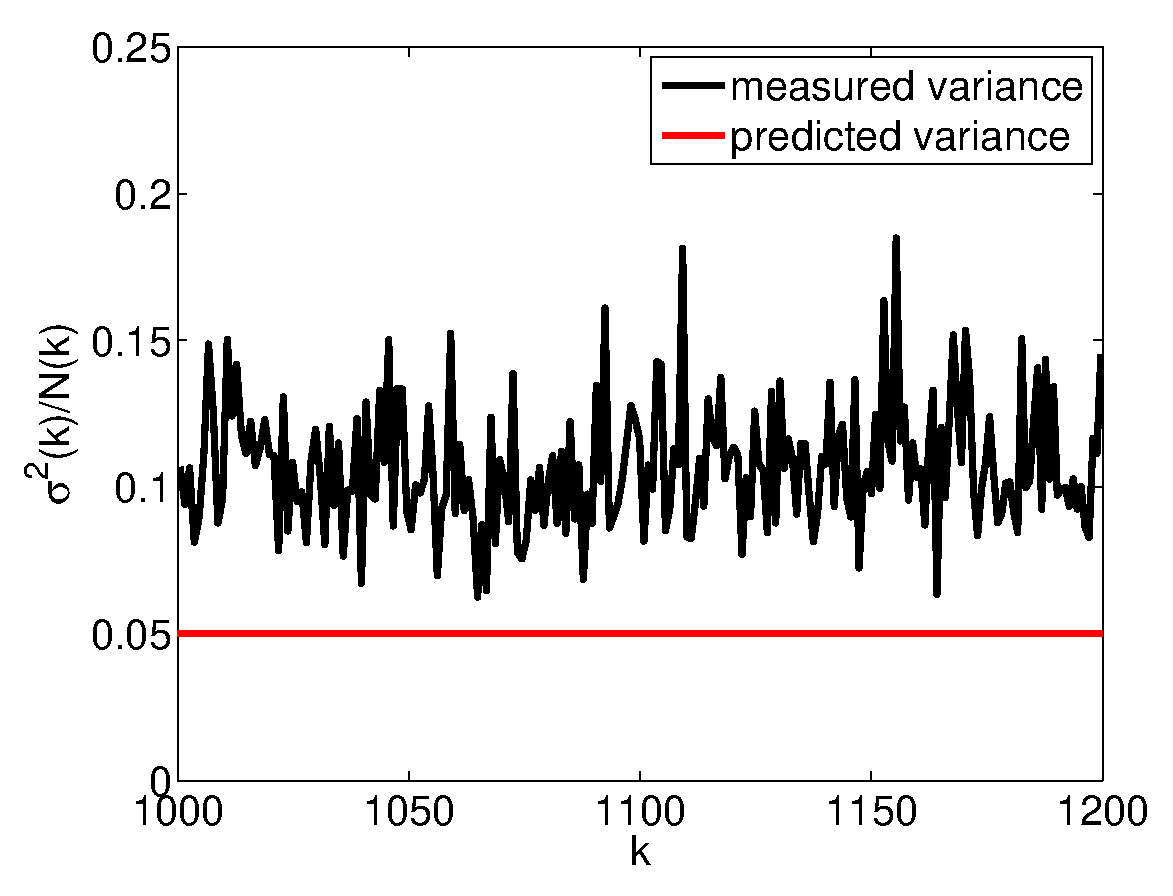
\includegraphics[width=0.9\textwidth]{figs/results/qugrs_1000_to_1200_variance.eps}
    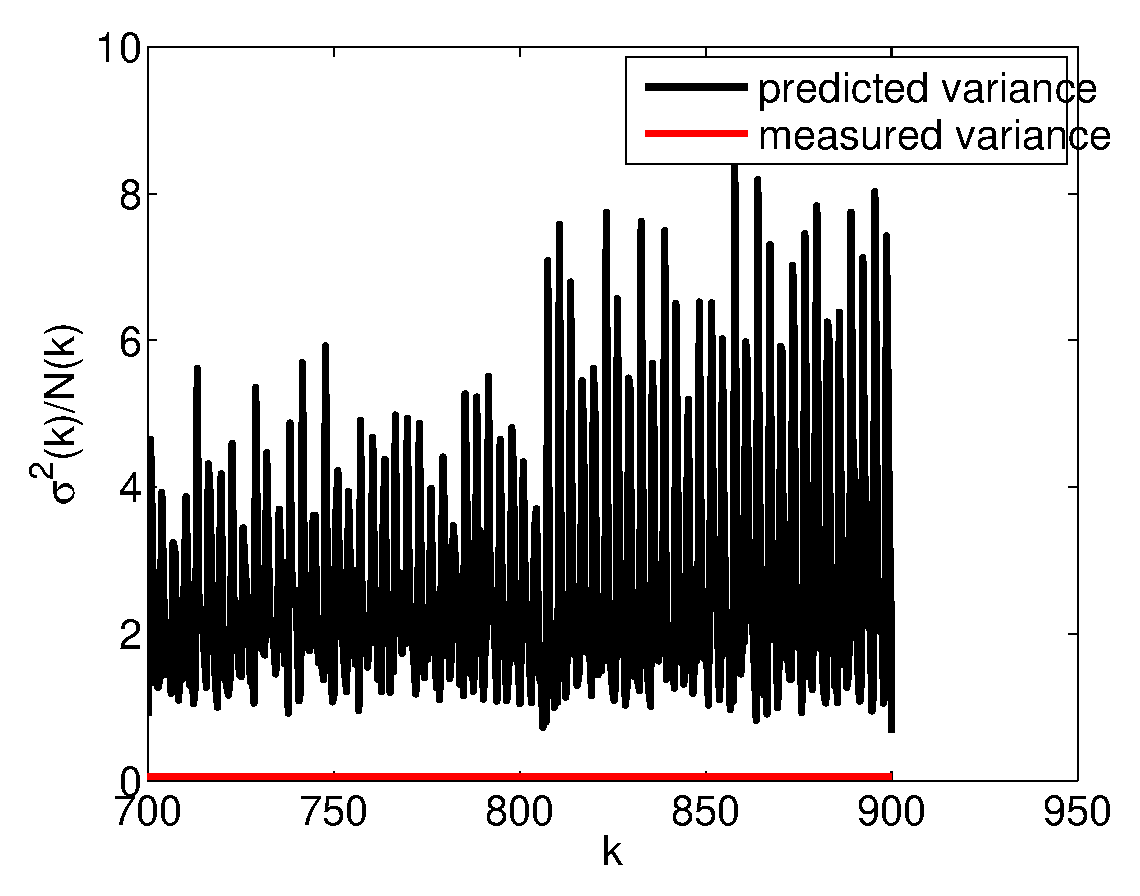
\includegraphics[width=0.9\textwidth]{figs/results/qust_700_to_900_variance.eps}

    \caption{Variance of number of nodal domains. Top: Sinai; middle: stadium; bottom: percolation}
    \label{fig:variance}
  \end{center}
\end{figure}

\begin{figure}
  \begin{center}
    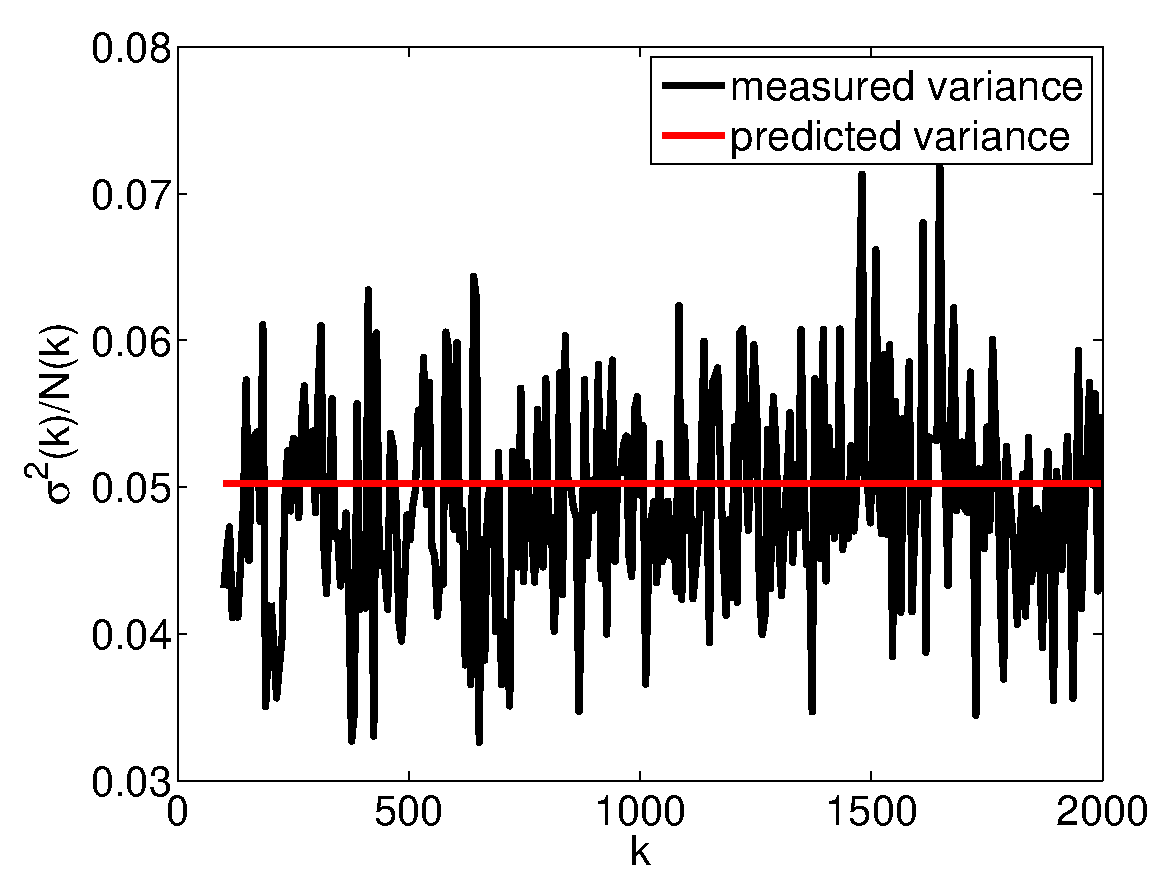
\includegraphics[width=\textwidth]{figs/results/perc_100_to_2000_variance.eps}
  \end{center}
\end{figure}

\section{Distribution of number of nodal domains}
The number of nodal domains for the Sinai billiard is nearly normal with a slight left skew (fig. \ref{fig:histograms}).

\begin{figure}
  \begin{center}
    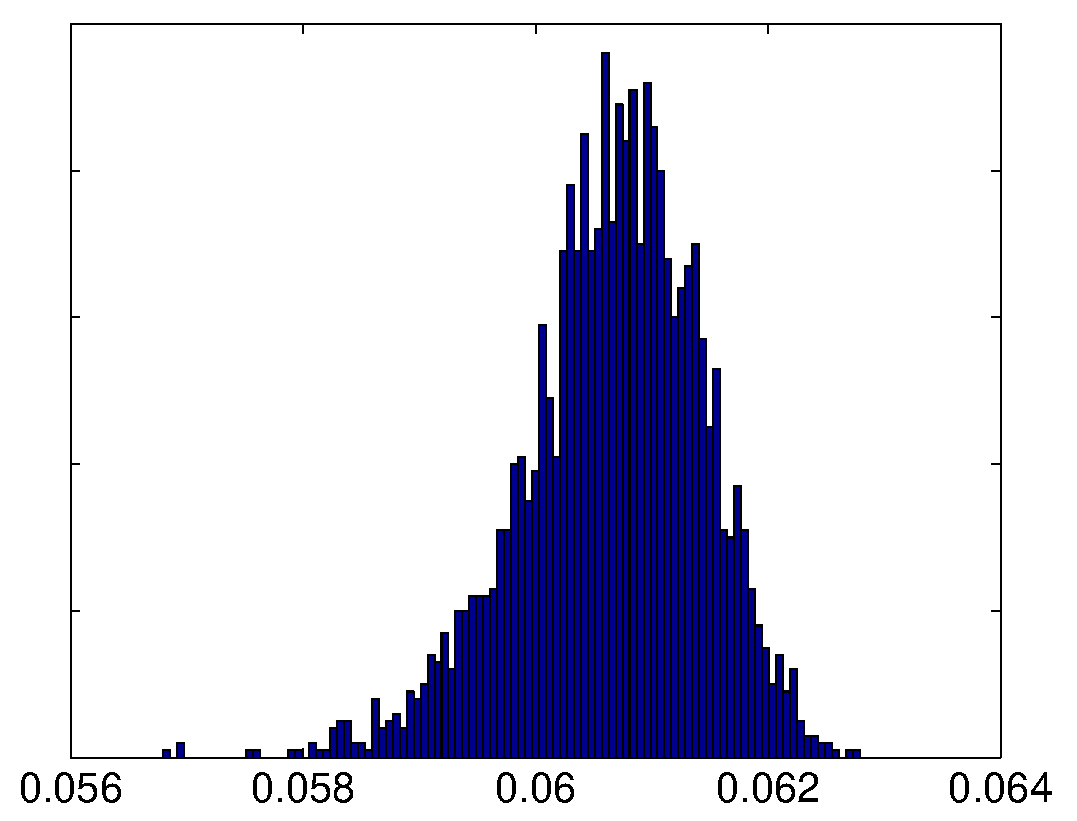
\includegraphics[width=0.8\textwidth]{figs/results/qugrs_2000_to_2020_count_histogram.eps}
    \linebreak
    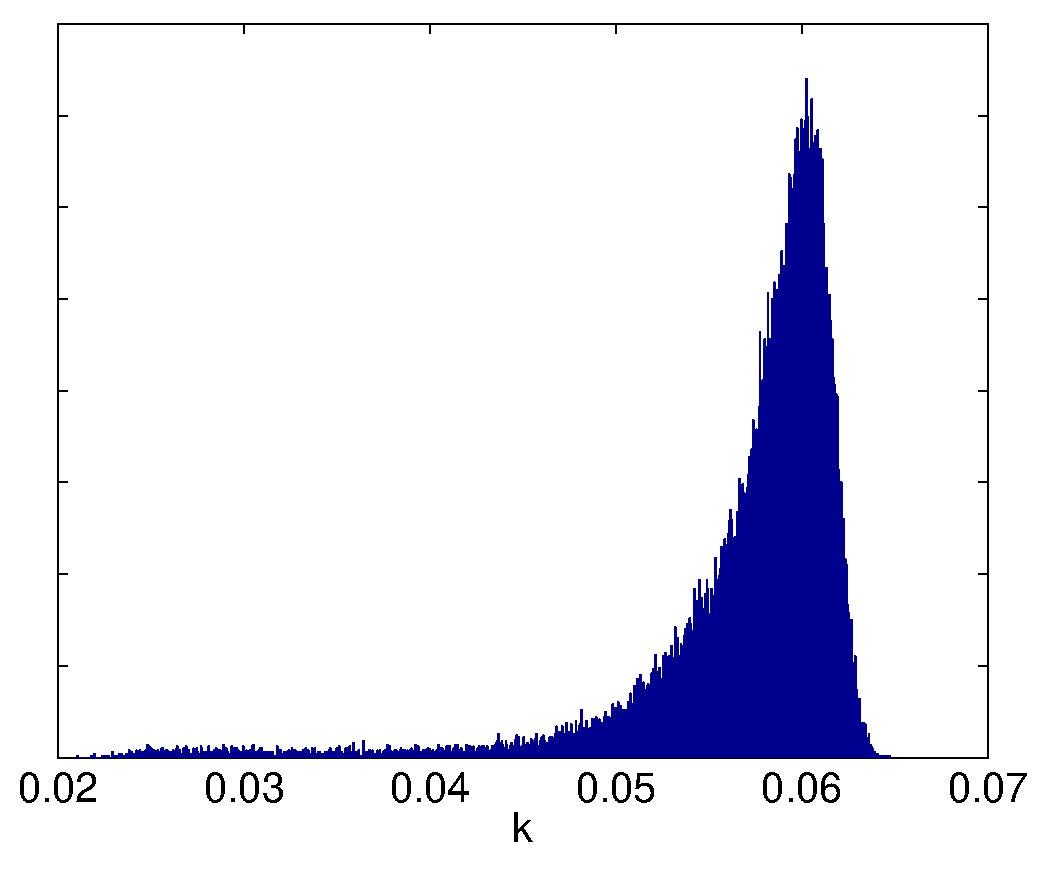
\includegraphics[width=0.8\textwidth]{figs/results/qust_700_to_900_count_histogram.eps}
    \caption{Histogram of scaled nodal domain counts. Above: Sinai billiard with $k \in [2000, 2020]$; below: stadium billiard with $k \in [700, 900]$.}
    \label{fig:histograms}
  \end{center}
\end{figure}

There is a strong left skew in the distribution of nodal domain counts in the stadium billiard (fig. \ref{fig:histograms}). This is due to bouncing ball modes (fig. \ref{fig:bouncing_ball_mode}), which have much fewer nodal domains than general chaotic eigenfunctions (fig. \ref{fig:wtms}). Bouncing ball modes have a high concentration of probability mass in the central rectangular region and are largely responsible for the significantly lowered mean and large variance of nodal domain counts in the quarter stadium billiard. We can therefore identify bouncing ball modes by low probability mass in the quarter circle region. Specifically, we use the ``wing tip mass''
\[
w = \int_{W} u^{2}(\rr) d\rr
\]
where $W = \left\{ (x,y) \in \Omega \, \vert \, x \ge 1.1 \right\} $.

\begin{figure}
  \begin{center}
    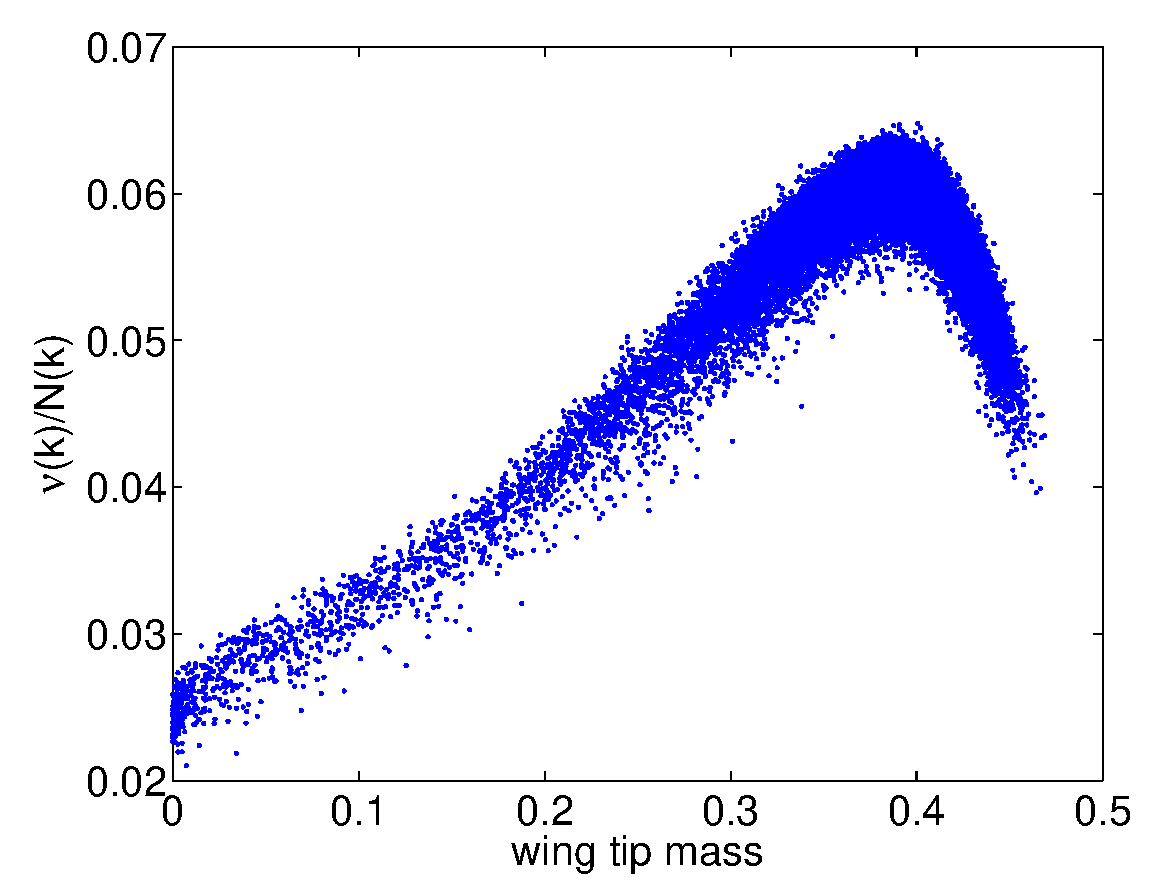
\includegraphics[width=\textwidth]{figs/results/qust_700_to_900_wtms.eps}
    \caption{Wing tip masses of eigenfunctions of the stadium billiard with $k \in [700, 900]$. The low wing tip mass regions have low nodal counts and skew the overall distribution while lowering the mean.}
    \label{fig:wtms}
  \end{center}
\end{figure}

\section{Areas of nodal domains}
The distribution of area of nodal domains all follow a power law. Nodal domain areas are scaled by the area of the smallest possible nodal domain $s_{min} = \pi (j_{1} / k)^{2}$ where $j_{1} \approx 2.4048$ is the first zero of the Bessel function $J_{0}$. The best fit exponent for the Sinai billiard is $2.0567 \pm 8.5524e{-4}$, which has a relative error of $8.65e{-4}$ and a difference of $2.079 \sigma$ from the conjectured value. For the stadium billiard, the best fit exponent is $2.0578 \pm 1.2e{-3}$, a $0.14\%$ error and a difference of $2.3 \sigma$. These deviations of order $2 \sigma$ are not statistically significant; thus we accept conjecture \ref{conj:area} for both billiard shapes.

\begin{figure}
  \begin{center}
    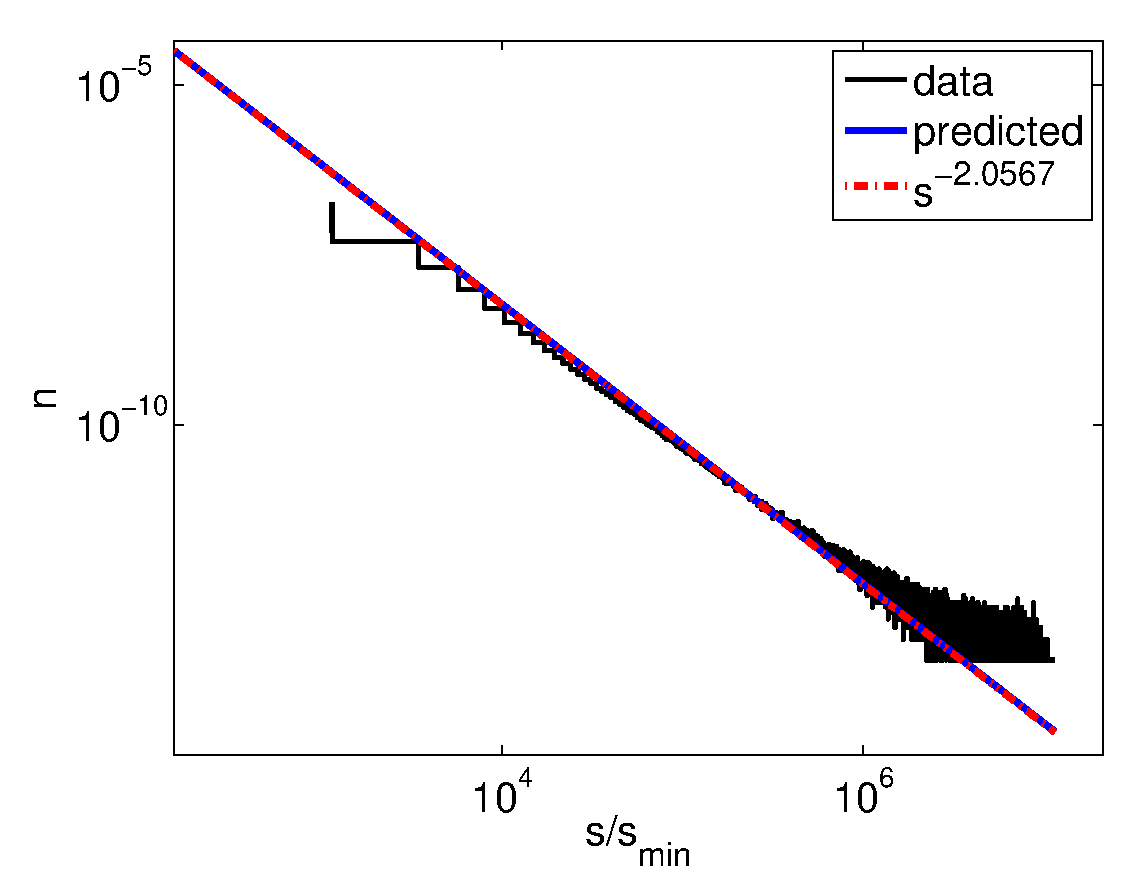
\includegraphics[width=0.8\textwidth]{figs/results/qugrs_1000_to_1100_sizes.eps}
    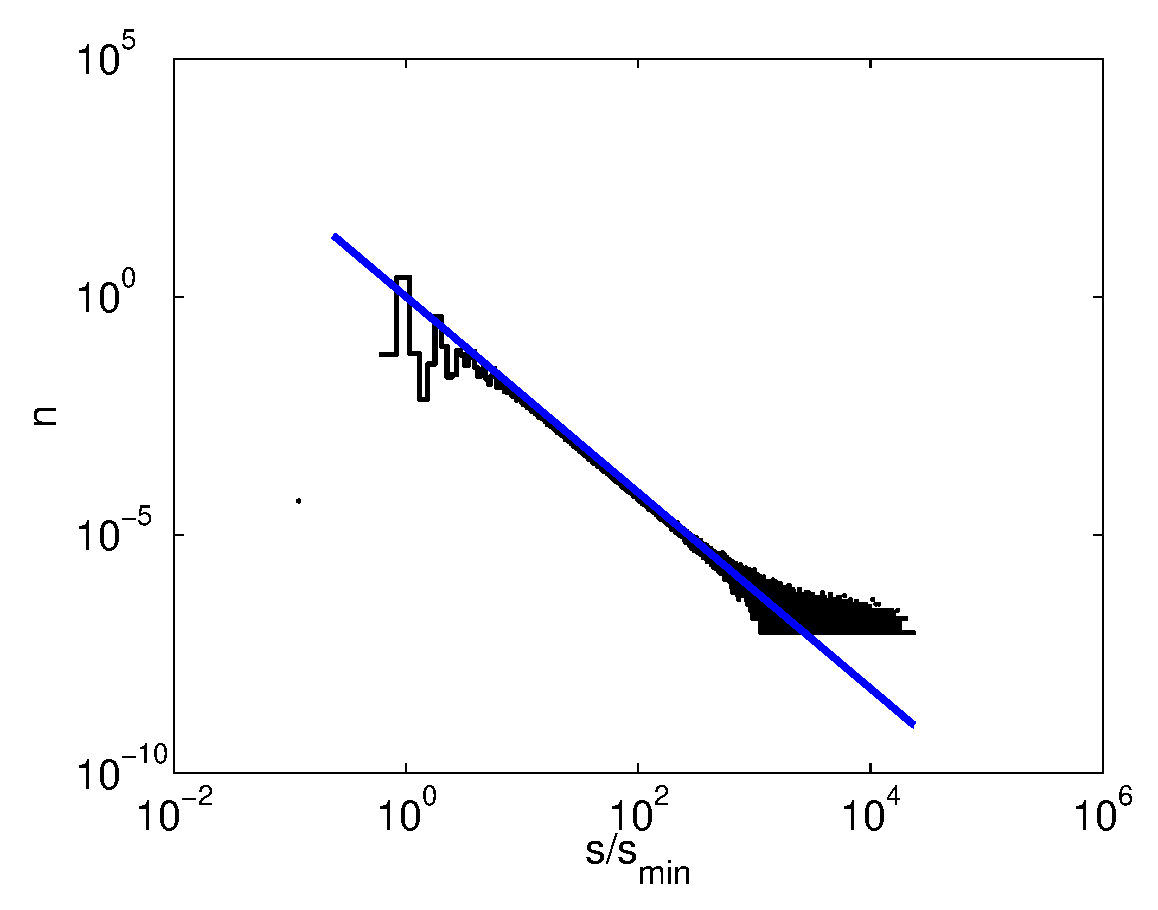
\includegraphics[width=0.8\textwidth]{figs/results/qust_700_to_900_sizes_0.1_sampled.eps}
    \caption{Relative frequencies of normalized nodal domain areas. The dashed red line shows the least-squares best fit of the form $s^{-\tau}$. Above: Sinai; below: stadium}
    \label{fig:area}
  \end{center}
\end{figure}

\chapter{Conclusion}
By combining the scaling method of Vergini and Saraceno \cite{vergini} with adaptive interpolation, we have obtained nodal domain data at energies 400 times higher than previously explored for over 100 times as many eigenfunctions as previously examined \cite{bogomolny07}. Comparing this data to the predictions of Bogomolny and Schmit \cite{bogomolny} from the percolation model, we find a that the distribution of sizes of nodal domains matches, while the mean and variance of number of nodal domains differ. We are the first to collect data from the generalized Sinai billiard, which displays hard chaos and has a mean number of nodal domains nearly in agreement with that determined experimentally for random superpositions of plane waves.

The source code for tools developed here has been released under an open source license \cite{gpl} and is available for the community to modify and distribute \cite{github}.

\appendix
\chapter{Definition of Ergodicity}
\label{sec:ergodicity}

Informally, a mapping $T$ is said to be ergodic if it has homogenous dynamics across its domain, i.e., there are no regions which behave ``differently'' under the mapping $T$. Formally, we consider $T$ as a mapping on a probability space. A probabilty space requires a measure, which is defined over a $\sigma$-algebra. Thus we present the following definitions:

\newtheorem{dfn}{Definition}
\begin{dfn}[$\sigma$-algebra]
$\Sigma \subset 2^{\Omega}$ is a \emph{$\sigma$-algebra} over $\Omega$ if:
\begin{enumerate}
\item
$\emptyset, \Omega \in \Sigma$
\item
$\Omega \backslash A \in \Sigma \; \forall A \in \Sigma$
\item
\[
\bigcup_{i=1}^{\infty}A_{i} \in \Sigma \; \forall \left\{A_{i}\right\}_{i=1}^{\infty}\text{ such that }A_{i} \in \Sigma \forall i
\]
\end{enumerate}
\end{dfn}

\begin{dfn}[Measure]
$\mu$: $\Sigma \rightarrow \mathbb{R}$ is a \emph{measure} on $\Sigma$ if:
\begin{enumerate}
\item
$\mu(A) \ge 0 \; \forall A \in \Sigma$
\item
$\mu(\emptyset) = 0$
\item
\[
\mu\left(\bigcup_{i=1}^{\infty} A_{i} \right) = \sum_{i=1}^{\infty} \mu(A_{i})
\]
\end{enumerate}
\end{dfn}

\begin{dfn}[Measure space]
A \emph{measure space} is a triple $(\Omega, \Sigma, \mu)$ where $\Sigma$ is a $\sigma$-algebra over $\Omega$ and $\mu$ is a measure on $\Sigma$.
\end{dfn}

\begin{dfn}[Probability space]
A \emph{probability space} is a measure space $(\Omega, \Sigma, \mu)$ where $\mu(\Omega) = 1$.
\end{dfn}

These definitions allow us to formally define ergodicity as:

\begin{dfn}[Ergodicity]
Let $(\Omega, \Sigma, \mu)$ be a probability space. A mapping $T$: $\Sigma \rightarrow \Sigma$ is \emph{ergodic} if $T(E) = E \implies \mu(E) = 0$ or $\mu(E) = 1$
\end{dfn}

Thus, under an ergodic mapping $T$, any $E \in \Sigma$ that maps to itself must have measure zero (in which case dynamics on this set are inconsequential) or measure one (in which case the set is almost the entire domain $\Omega$). Futhermore, all $E \in \Sigma$ such that $0 < \mu(E) < 1$ must contain points that map to points outside of $E$ under $T$. In this sense, $T$ ``mixes'' points in the domain $\Omega$.

\chapter{General Solution of the Helmholtz Equation}
\label{sec:helmholtz_basis}
Here we show that the functions $J_{n}(k r) \sin(n \theta)$ and $J_{n}(k r) \cos(n \theta)$ form a complete basis of solutions of (\ref{eq:helmholtz}).

In polar coordinates,
\[
\Delta = \frac{1}{r} \partial_{r} (r \partial_{r}) + \frac{1}{r^{2}} \partial_{\theta \theta}
\]
Thus, (\ref{eq:helmholtz}) can be expressed as
\[
u_{rr}(r, \theta) + \frac{1}{r} u_{r}(r, \theta) + \frac{1}{r^{2}} u_{\theta \theta}(r, \theta) + k^2 u(r, \theta) = 0
\]
Using separation of variables we attempt solutions of the form
\[
u(r, \theta) = R(r) \Theta(\theta)
\]
where $\Theta(\theta)$ is periodic with period $2 \pi$. This gives
\[
\Theta''(\theta) + n^{2} \Theta(\theta) = 0
\]
and
\[
r^{2} R''(r) + r R'(r) + r^{2} k^{2} R(r) - n^{2} R(r) = 0
\]
The periodicity of $\Theta(\theta)$ requires that
\[
\Theta(\theta) = \alpha \sin(n \theta) + \beta \cos(n \theta)
\]
where $n \in \mathbb{Z}$.
The radial differential equation is known as Bessel's equation and has solutions
\[
R(r) = J_{n}(k r)
\]
where $J_{n}$ is a regular Bessel function and $k \in \mathbb{R}$ is allowed to take discrete values determined by boundary conditions.

Thus, the general solution of (\ref{eq:helmholtz}) can be expressed as a sum of the form

\begin{equation}
  \label{eq:helmholtz_gen_soln}
  b_{0} J_{0}(kr) + \sum_{n = 1}^{\infty}{a_{n} J_n(kr) \sin{n \theta} + b_{n} J_n{kr} \cos{n \theta}}
\end{equation}


\comment{
\chapter{Code Interface}
\label{sec:api}
Code implementing Vergini's scaling method to compute eigenfunctions was written by Alex Barnett. Code for counting nodal domains was written by the author. All code used herein is open source and available under the GPL license \cite{gpl} \cite{github}. Appendix \ref{sec:api} contains an overview of the functions provided by this library.

\section{Command Line Interface}
\subsection{Verg}
The verg program uses the scaling method described in \ref{sec:scaling_method} to find eigenvalues and eigenfunctions of the Laplace operator on domains in $\mathbb{R}^{2}$.

\begin{verbatim}
verg -l qust:2 -b 10 -s vepwoo:1.2:40:1.5 -k 200.01 -V 0.005 -f 0.001 -m
verg -l qugrs:1:0.4:0.7 -s oyooo:1.5:7:1 -u -4 1 -k 200.1 -V 0.005 -f 0.001 -m
\end{verbatim}


\subsection{Count}
\begin{verbatim}
count -f t.sta_bin -m t.mask.sta_bin -l qust:2 -d .001 -k 200.01 -M 8 -u 20
\end{verbatim}
The count program counts nodal domains over a domain in $\mathbb{R}^{2}$ using the adaptive interpolation scheme described in \ref{sec:interpolation}.

\subsection{Vc}
\begin{verbatim}
vc -n run_2018.450000 -l qugrs:1.0:0.4:0.7 -s oyooo:1.5:7:1 -u -4 1 -k 2018.450000 -V 0.050000 -d 0.000347 -M 9 -p 30
\end{verbatim}
The vc program combines verg and count to compute eigenfunctions and count their nodal domains.

\subsection{Perc}
\begin{verbatim}
perc -r 100:6:1000 -N 100
\end{verbatim}
The perc program generates random grids using the percolation model described in \ref{sec:percolation} and counts the nodal domains in the generated grids.
}

\bibliographystyle{plain}
\bibliography{thesis}

\end{document}
